\section{Spectra are your friends (Rok Gregoric)} 
This is a minicourse on stable homotopy theory, specifically spectra, taught by Rok Gregoric. The word ``spectra'' (or spectrum) shows up so much in math, for example the spectrum of an operator in functional analysis, the spectrum of a commutative ring in algebraic geometry, and spectra as a basic object of study in stable homotopy theory. The first two ideas are closely related while the third idea less so. 

This minicourse will use $\infty$-categories as a warning to the faint of heart readers. As for prerequisites, it would be nice to know some algebraic topology (homotopy and homology) and a little bit of category theory. However, no background in stable homotopy theory will be assumed. The course will not prove much, the standard reference is \cite{lurie}.

\subsection{$\infty$-categories, loops, and suspension (May 24)}
As an introduction, a story says that mathematics began with shepherds counting sheep by enumerating elements of $\Z_{\geq 0}=\N$. Adding two flocks of sheep induced a monoid (group without inverses) structure $\Z_{\geq 0}\times \Z_{\geq 0}\to  \Z_{\geq 0}$, and negative numbers came about by the group completion of the monoid $(\Z_{\geq 0})^{\mathrm{gp}}=\Z$. 
After the integers, we figured out how to multiply and got a ring structure. From here we obtain the abelian groups as the category of modules over the integers $(\mathsf{Ab} \simeq \mathsf{Mod} _{\Z})$, and everything in algebra follows. This is how algebra came about, and this is where we supposedly went wrong: we should have been working with the sphere spectrum all along.
%\begin{figure}[H]
%\centering
 %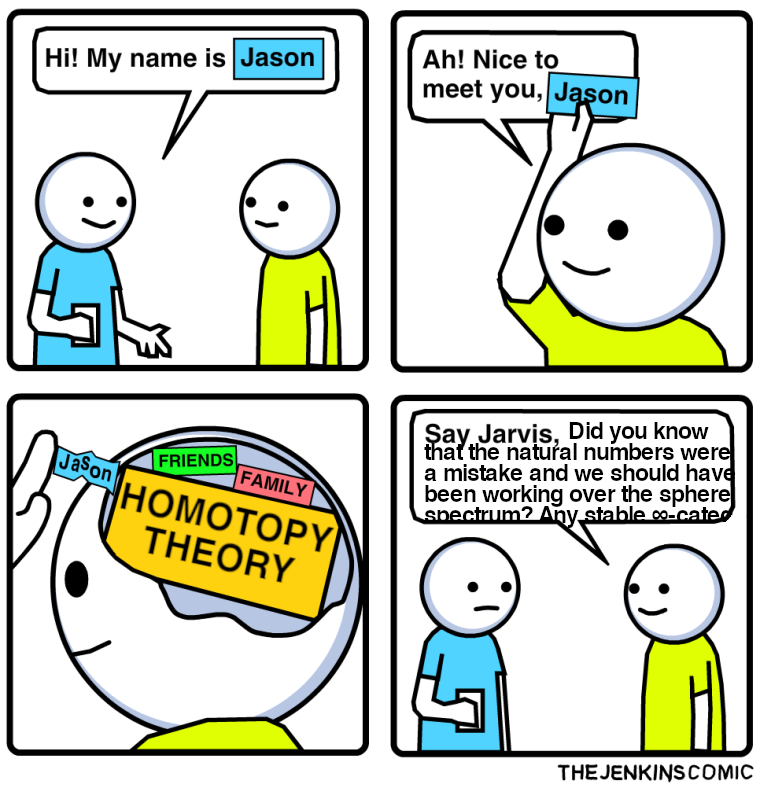
\includegraphics[width=0.5\linewidth]{figures/jarvis.png}
 %\label{jarvis} 
 %\caption{A relevant meme.} 
%\end{figure}

What if instead of considering equivalent classes of sheep, the shepherds remembered they could ``change'' the sheep, for example saying ``this is sheep 1 and sheep 2, but I can rename sheep 1 to sheep 2 and vice versa''? Instead of using equivalence classes of finite sets up to bijection, what if the shepherds remembered bijections as well? So if we worked with finite sets up to bijection (the category $\mathsf{Fin} ^{\simeq}$), we can pass to $\N$ by the cardinality function $|\cdot |$, which is not a drastic change. The claim is we arrive at the sphere spectrum by imitating the historical development of the integers.

We have somewhat of a monoid structure by taking the disjoint union of finite sets $\mathsf{Fin} ^{\simeq} \times \mathsf{Fin} ^{\simeq}\to \mathsf{Fin} ^{\simeq},$ where $(I,J) \mapsto I \amalg J$. With the sufficient theory, we can consider the group completion $S :=(\mathsf{Fin} ^{\simeq})^{\mathrm{gp}}$, which is an incarnation of the \textbf{sphere spectrum}. There is a natural multiplication $(I,J) \mapsto I \times J$ which, passing by cardinalities to the integers, is just the natural product. So $S$ is a ring, and we can form $\mathsf{Sp} := \mathsf{Mod} _S$, the category of modules over $S$. Voil\`a, this is what a spectra is. This is an intuitive perspective and we glossed over many things, we will come back and clarify much of this later on.


Another story: an Indian emporer asked many blind men to touch and elephant and report back on what it is. Each blind man touched a different part of the elephant like the snout or leg, and thus reported back thinking they had found a tree or a sword or whatever. None of them had the complete picture, but each of them has said the truth. An elephant is quite complicated--- you could describe it as a collection containing the ears, the trunk, the tusks, etc. Each of these is an \textit{aspect} of the elephant, and in the same way spectra have many different incarnations:
\begin{itemize}
\setlength\itemsep{-.2em}
    \item (co)homology theories,
    \item spaces stable under suspension,
    \item infinite loop spaces,
    \item homotopy-coherent analogue of abelian groups,
    \item modules over the sphere spectrum $S$,
\end{itemize}
and so on.

%\orbreak
%\subsubsection*{$\infty$-categories in a nutshell} 
\begin{definition}[]
    An $\mathbf \infty$\textbf{-category} $\mathcal{C} $ consists of:
    \begin{enumerate}[label=(\roman*)]
    \setlength\itemsep{-.2em}
        \item A set of objects $C \in \mathcal{C} $,
        \item Spaces of maps $\mathrm{Map}_{\mathcal{C} }(C,C') \in \mathcal{S} $ for all $C,C' \in \mathcal{C} $,
        \item A composition map \[
                \mathrm{Map}_{\mathcal{C} }(C',C'')\times \mathrm{Map}_{\mathcal{C} }(C,C') \to \mathrm{Map}_{\mathcal{C} }(C,C''),\quad (f,g) \mapsto f \circ g.
        \] which is associative and unital \emph{up to coherent homotopy}.
    \end{enumerate}
\end{definition}

\begin{figure}
\centering
\begin{tabular}{|| c | c ||} 
    \hline
    Classical math & Homotopical math \\
    \hline\hline
    equality ($=$) & equivalence ($\simeq$)\\ \hline
    sets $(\mathsf{Set} $) & $\underset{\text{(homotopy types, anima...)}}{\text{spaces (}\mathcal{S} \text{)}} $\\ \hline
    categories & $\infty$-categories \\ \hline
\end{tabular}
\label{comparison}
\caption{A comparison of ideas in classical math versus homotopical math.} 
\end{figure}

What do we mean by ``homotopy coherence''? Say we have two maps $f \circ (g \circ h)$ and $(f \circ g) \circ h$, these maps aren't actually equal, but equivalent. This equivalence $f \circ (g \circ h) \simeq (f \circ g) \circ h$ is a path in the space of maps $\mathrm{Map }_{\mathcal{C} }(C,C'')$. Given a triple composition $((f \circ g) \circ h) \circ k$, there are several different ways to express this, and chaining the homotopies that encode their equivalence gives a ``loop'' in a mapping space of sorts. This mapping space may give different (non-unique) choices of expression, which is bad, so homotopy coherence specifies that we can express composition up to contractible mapping spaces (so a unique choice). In essence, we can write expressions like $f \circ g \circ h$ without brackets, since it's unique up to contractible ambiguity.
For example, when we say the following diagram commutes, \[
\begin{tikzcd}
    \bullet \arrow[d,"f"']\arrow[dr,"h"]& \\
    \bullet \arrow[r,"g"']& \bullet
\end{tikzcd}
\] this implies that $h\simeq g \circ f$. This homotopy is implictly constructing a 1-simplex with the vertices of the triangle, and ``filling'' in the simplex to make the space contractible. This means that we have many choices of composite morphisms (the paths going through the middle), and they're all related by contractible ambiguity.

\begin{example}
    What are some key examples of $\infty$-categories?
    \begin{itemize}
\setlength\itemsep{-.2em}
        \item An ordinary (locally small) category is an $\infty$-category where the mapping spaces are just discrete topologies (sets).
        \item The spaces $\mathcal{S} $ form an $\infty$-category.
        \item $\mathsf{Cat} _{\infty}$ is an $\infty$-category of $\infty$-categories.
    \end{itemize}
\end{example}
The cool thing is that we can pass much of category theory through the language of $\infty$-categories. This is where we gloss over things a little bit--- proving all of category theory for $\infty$-categories is hard, and some other people (Jacob Lurie and Emily Riehl, see \cite{lurie} ) have already done all of it.
\begin{example}
    Here are some familiar notions from category theory.
    \begin{itemize}
\setlength\itemsep{-.2em}
        \item The \textbf{initial object} $C \in \mathcal{C} $ is an object such that $\mathrm{Map}_{\mathcal{C} } (C,C')$ is contractible for all $C' \in \mathcal{C} $. Terminal objects are similarly defined. For example, in $\mathcal{S} $ (the $\infty$-category of spaces), the initial object is the empty space and terminal objects are contractible spaces.
        \item For $C \in \mathcal{C} $, we define the \textbf{overcategory} $\mathcal{C} /C$ with objects as morphisms $C' \to C$. A map in $\mathrm{Map}_{\mathcal{C} /C}(C' \to C, C''\to C)$ makes the following diagram commute: \[
        \begin{tikzcd}
            C' \arrow[rr]\arrow[rd]& & C''\arrow[ld] \\
               & C &
        \end{tikzcd}
        \] Undercategories $C / \mathcal{C} $ are defined analogously.
    \item An example of these constructions are \textbf{pointed spaces} $\mathcal{S} _*$, defined as the undercategory $* / \mathcal{S} $ of a contractible space. So morphisms between objects of pointed spaces $(x \colon * \to X) \in \mathcal{S} _*$ have to preserve the basepoint $*$.
    \item \textbf{Functors} also make sense, where the maps between morphisms are compatible with all the higher homotopies between them. This also gives rise to the $\infty$-category of functors.
    \item \textbf{Limits} and \textbf{colimits} give rise to \textbf{homotopy limits} (and \textbf{homotopy colimits}), and they have universal properties! For intuition on limits and colimits, consider a functor from the integers by comparison to a category $\mathcal{C} $. \[
            \underset{\text{functor} \ F \colon (\Z,\geq ) \to \mathcal{C} }{\underbrace{  \overset{\varprojlim F(n)}{\bullet} \longrightarrow \cdots \longrightarrow\overset{F(-3)}{\bullet } \longrightarrow \overset{F(-2)}{\bullet} \longrightarrow \overset{F(-1)}{\bullet} \longrightarrow \overset{F(0)}{\bullet} \longrightarrow \overset{F(1)}{\bullet } \longrightarrow \overset{F(2)}{\bullet} \longrightarrow \overset{F(3)}{\bullet} \longrightarrow \cdots \longrightarrow \overset{\varinjlim F(n)}{\bullet} }} 
        \] A \emph{diagram} is just this functor $F$. Then a colimit (denoted $\varinjlim$) is the farthest thing you can put on the right, and a limit (denoted $\varprojlim$) is the farthest thing you can put on the left. Unlike analysis, we don't need a linear diagram, we just need to find the farthest things on the left/right of some diagram.
    \end{itemize}
    Here are two examples of limits and colimits. Suppose we have a terminal object $* \in \mathcal{C} $. Then the \textbf{suspension} of $C \in \mathcal{C} $ (denoted $\Sigma C)$ is the pushout $* \amalg_C *$ of $C \to *$ with itself, or the colimit that completes the diagram on the left.
    \[
    \begin{tikzcd}
        C\arrow[r]\arrow[d] & *\arrow[d] \\
        *\arrow[r] & \Sigma C\arrow[ul,phantom,"\ulcorner", very near start]
    \end{tikzcd}\qquad\qquad
    \begin{tikzcd}
        \Omega C\arrow[d]\arrow[r] \arrow[dr,phantom,"\lrcorner",very near start]& *\arrow[d] \\
        *\arrow[r] &C
    \end{tikzcd}
\] 
Similarly, given an initial object $* \in \mathcal{C} $, the \textbf{(based) loops} on $C \in \mathcal{C} $ are defined as the pullback $\Omega C:= * \times_C  *$, the limit that completes the diagram on the right.
\begin{itemize}
\setlength\itemsep{-.2em}
    \item \textbf{Adjunctions} between categories $\mathcal{C} ,\mathcal{D} $ consist of two functors $F \colon \mathcal{C}  \to \mathcal{D} ,\ G \colon \mathcal{D}  \to \mathcal{C} $ such that \[
            \mathrm{Map}_{\mathcal{D} }(F(C),D)\simeq \mathrm{Map}_{\mathcal{C} (C, G(D))}
    \] for all $C \in \mathcal{C} ,\ D \in \mathcal{D} $. This relation is denoted $F\dashv G$. We say $F$ is a \textbf{right adjoint functor} while $G$ is a \textbf{left adjoint functor}. A basic yet profound fact in category theory is that left adjoints preserve colimits while right adjoints preserve limits.
\end{itemize}
\end{example}

\begin{claim}
    Let $\mathcal{C} $ be an $\infty$-category with a zero object\footnote{A zero object is just an object that is both initial and terminal.} $*$. Then $\Sigma \dashv \Omega$.
\end{claim}
\begin{proof}
    The claim is that $\mathrm{Map}_{\mathcal{C} }(\Sigma C, C')\simeq \mathrm{Map}_{\mathcal{C} }(C,\Omega C')$. How do we show this? Since colimits factor out of $\Hom$ to become limits, or more precisely $\Hom(\varinjlim F, N)=\varprojlim \Hom(F-,N) $, we have
    \begin{align*}
        \mathrm{Map}_{\mathcal{C} }(\Sigma C,C')&\simeq \mathrm{Map}_{\mathcal{C} }(*\amalg_C *, C')\\
                                                &\simeq \mathrm{Map}_{\mathcal{C} }(* , C') \times _{\mathrm{Map}_{\mathcal{C} }(C,C')} \mathrm{Map}_{\mathcal{C} }(*, C') \quad \text{\small by factoring out colimits} \\
                                                &\simeq \mathrm{Map}_{\mathcal{C} }(C,*) \times_{\mathrm{Map}_{\mathcal{C} }(C,C')}\mathrm{Map}_{\mathcal{C} }(C,*) \quad \text{\small by contractibility} \\
                                                &\simeq \mathrm{Map}_{\mathcal{C} }(C , * \times _C *) \\
                                                &\simeq \mathrm{Map}_{\mathcal{C} }(C,\Omega C').\qedhere
    \end{align*}
\end{proof}

\begin{definition}[]
    A \textbf{homotopy category} of an $\infty$-category $\mathcal{C} $ is an ordinary 1-category $\mathrm{h} \mathcal{C} =\mathsf{Ho}(\mathcal{C})  $, where 
    \begin{align*}
        \mathrm{ob}(\mathsf{Ho} \mathcal{C} )&:= \mathrm{ob}(\mathcal{C} ),\\
        \Hom _{ \mathsf{Ho} \mathcal{C} }(C,C')&:= \pi_0 (\mathrm{Map}_{\mathcal{C} }(C,C')).
    \end{align*}In other words, the objects are just the objects of $\mathcal{C} $, and the path components of the mapping space $\mathrm{Map}_{\mathcal{C} }(C,C')$ forms the set of morphisms of $\mathsf{Ho} \mathcal{C} $. For topological spaces, this is your familiar category of spaces up to homotopy $\mathsf{hTop} $ from algebraic topology.
\end{definition}

\orbreak
This ends the ``$\infty$-category theory in a nutshell'' section of this minicourse. Now let's talk about stability.
\begin{definition}[]
    A (1-)category $\mathcal{C} $ is \textbf{abelian} if
    \begin{enumerate}[label=(\roman*)]
    \setlength\itemsep{-.2em}
        \item it has a zero object $0 \in \mathcal{C} $,
        \item it has a biproduct\footnote{A biproduct is both a product and a coproduct.} $\oplus$,
        \item every morphism $f \colon C \to C'$ has a kernel $\ker (f) \to C$ and a cokernel $C' \to \mathrm{coker}(f)$,
        \item for every $f \colon C \to C'$ in $\mathcal{C} $, $\coker (\ker (f) \to C)\simeq \ker(C' \to \coker (f))$. This is a generalization of the first isomorphism theorem, where if you think of $\coker(f)$ as $C' /\im f$, the RHS equals $\ker(C' / \im f)=\im f,$ while the LHS becomes $\coker(\ker f)= C /\ker f$. So $C /\ker f\simeq \im f$. Diagramatically, \[
        \begin{tikzcd}
\ker(f) \arrow[d] \arrow[r]      & 0 \arrow[d] \\
C \arrow[r, two heads] \arrow[u] & \coker(f)  
\end{tikzcd}
        \] is both a pullback and a pushout. You can also think of this as saying that limits and colimits coincide in certain cases.
    \end{enumerate}
\end{definition}
So how do we transport this notion to $\infty$-land?
\begin{definition}[]
    An $\infty$-category $\mathcal{C} $ is \textbf{stable} if
    \begin{enumerate}[label=(\roman*)]
    \setlength\itemsep{-.2em}
        \item it has a zero object $0 \in \mathcal{C} $,
        \item it has a biproduct $\oplus$,
        \item every morphism $f \colon C \to C'$ admits a \textbf{fiber}\footnote{A way of motiviating this terminology is by realizing the kernel is the fiber of 0.} (or \emph{homotopy kernel}) and \textbf{cofiber} (or \emph{homotopy cokernel}), where the fiber is the pullback of $f$ along the zero map, and the cofiber is the pushout of $f$ along the zero map. \[
        \begin{tikzcd}
            \mathrm{fib}(f)\arrow[r]\arrow[d] \arrow[dr,phantom,"\lrcorner",very near start]& 0 \arrow[d]\\
            C \arrow[r,"f"] & C'
        \end{tikzcd}\qquad\qquad     
        \begin{tikzcd}
            C\arrow[r,"f"]\arrow[d] & C' \arrow[d]\\
            0 \arrow[r] & \mathrm{cofib}(f)\arrow[ul,phantom,"\ulcorner", very near start]
        \end{tikzcd}
        \] 
    \item any $C'\to C \to C''$ in $\mathcal C$ is a \textbf{fiber sequence} (fits into the left diagram) iff it is a \textbf{cofiber sequence} (fits into the right diagram). In other words, the square \[
    \begin{tikzcd}
        C'\arrow[r]\arrow[d]\arrow[dr,phantom,"\lrcorner",very near start]& C\arrow[d]\\
        0\arrow[r]& C''\arrow[ul,phantom,"\ulcorner",very near start]
    \end{tikzcd}
    \]is a pullback iff it is a pushout.
    \end{enumerate}
\end{definition}

\begin{example}
    Any sequence $C \to 0 \to C'$ is a fiber if $C \simeq 0 \times_{C'}0\simeq \Omega C' $, and a cofiber if $C'\simeq 0 \amalg_C 0\simeq \Sigma C$. This tells us that in stable $\infty$-categories, we can ``undo'' the suspension to get loops, and vice versa. This gives an equivalent characterization of stability--- $\mathcal{C} $ with a zero object is stable iff 
\begin{itemize}
\setlength\itemsep{-.2em}
    \item it has all finite limits,
    \item $\Omega \colon \mathcal{C} \overset{\sim}{\to} \mathcal{C}  $,
\end{itemize}or iff
\begin{itemize}
\setlength\itemsep{-.2em}
    \item it has all finite colimits,
    \item $\Sigma\colon \mathcal{C} \overset{\sim}{\to} \mathcal{C}  $,
\end{itemize}or iff
\begin{itemize}
\setlength\itemsep{-.2em}
    \item it has all finite limits and colimits,
    \item any square \[
    \begin{tikzcd}
        C'\arrow[r]\arrow[d]& C\arrow[d]\\
        0\arrow[r]& C''
    \end{tikzcd}
    \] in $\mathcal{C} $ is a pullback iff it is a pushout.
\end{itemize}
Since these two functors are adjoint, if either one exists the other characterization holds, or $\Omega\simeq \Sigma ^{-1}$. So stability tells us that loops and suspension are not just in adjunction, but in \emph{equivalence}. This means we study things \emph{stable} under loops or suspension, hence the nomenclature.
\end{example}

\begin{example}
    The $\infty$-category $\mathcal{S}_* $ is not stable. There is no biproduct, and the initial object $(\O)$ and the terminal object $(\{*\} )$ are not the same. To fix this, consider pointed spaces to get a zero object, and you can think about biproducts in your free time. We have (finite) limits and colimits in $\mathcal{S} _*$, however, $\Omega,\Sigma \colon S_* \to S_*$ are not equivalences. To see this, consider $X$ any non-based space and $X_+ =X\amalg \{*\} \in \mathcal S_* $. Then loops $\Omega X_+ \simeq *$ because loops are pointed at $\{*\} $, and ``undoing'' loops means we can get back information about $X$, which should not be the case.
    
    For example, we only have one map $S ^2 \to S^1 $, where $\pi_2(S^1 )=0$. However, suspending this results in a map $S^3\to S^2$, including the Hopf fibration ($\pi_3(S^2)\simeq \Z )$. Then desuspending kills the Hopf fibration.
\end{example}
\orbreak
The big idea is this: spaces are generally not stable, and to fix this lack of stability, we introduce spectra. How do we fix this? With spectra. The idea is to ``make $\Omega$ invertible by force''. Define the $\mathbf \infty$\textbf{-category of spectra} as the inverse limit \[
    \mathsf{Sp}:= \varprojlim \big( \cdots  \overset{\Omega}{\longrightarrow} \mathcal S_*\overset{\Omega}{\longrightarrow} \mathcal S_*\overset{\Omega}{\longrightarrow} \mathcal S_*\overset{\Omega}{\longrightarrow} \mathcal S_*\big),
\] then the $\infty$-category of spectra has finite limits, and  will respect $\Omega \colon \mathcal{S} _* \overset{\sim}{\to}  \mathcal{S_*} $.

\subsection{Spectra and stabilization (May 25)}
Some observations on the definition of spectra:
\begin{itemize}
\setlength\itemsep{-.2em}
    \item The category of spectra is a \emph{limit} formed in the $\infty$-category of $\infty$-categories ($\mathsf{Cat} _{\infty}$), and hence a category. Each $\Omega$ is a functor between categories, where objects in $\mathsf{Cat} _{\infty}$ are the $\infty$-categories $\mathcal{S} _*$.
    \item $\mathsf{Sp} $ is a stable $\infty$-category by design, or $\Omega \simeq \Sigma ^{-1}$.
    \item A \textbf{spectrum}, i.e. an object $X \in \mathsf{Sp} $, consists of spaces $X_i $ associated to each $\mathcal{S} _*$ with equivalences $X_i \simeq \Omega X_{i+1}$ for all $i \in \Z$. If you've read \emph{War and Peace} (the literature) on spectra, the equivalence $X_i\simeq \Omega X_{i+1} $ holds for $\mathbf \Omega$\textbf{-spectra}. There is an analogous notion of a $\mathbf \Sigma$\textbf{-spectra} (or ``pre-spectra''), defined as a collection of pointed spaces $X_i \in \mathcal{S} _* $ with pointed maps $\Sigma X_i  \to X_{i+1}$. The difference between these two notions is we do not require the structure maps $\Sigma X_i  \to X_{i+1}$ to be homotopy equivalences.
\end{itemize}

\begin{example}
    Let $X \in \mathcal{S} _*$. Then we can form the \textbf{suspension spectrum} $\Sigma ^{\infty}X \in \mathsf{Sp} $ as a $\Sigma$-spectrum, where $\left( \Sigma ^{\infty}X \right) _i :=\Sigma^i  X$ for all $i\geq 0$, where $\Sigma^i X$ is the $i$th suspension of $X$. The structure maps are then given by \[
        \Sigma\left(\Sigma ^{\infty}X\right)_i \simeq \Sigma \left( \Sigma^i X \right) \simeq \Sigma ^{i+1}X\simeq \left( \Sigma ^{\infty}X \right) _{i+1}.
    \] This is organically a $\Sigma$-spectrum and \emph{not} an $\Omega$-spectrum. Two example of suspension spectrum include the \textbf{zero spectrum} $0\simeq \Sigma ^{\infty}*$, and the \textbf{sphere spectrum} $S:=\Sigma ^{\infty}S^0,$ so that $\left( \Sigma ^{\infty}S\right) _i   \simeq S^i.$
\end{example}
\begin{figure}[h]
    \centering
\begin{tabular}{|| c || c | c || } 
   \hline& $\Omega$-spectra & $\Sigma $-spectra \\ \hline\hline
    PROS & $\infty$-categorically meaningful & easier to find component spaces\\ \hline
    CONS & more esoteric (complicated) & morphisms hard to define correctly \\ \hline
\end{tabular}
\label{procon} 
\caption{The pros and cons of $\Omega$-spectra and $\Sigma$-spectra.} 
\end{figure}
$\Omega$-spectra arose naturally as a way to make $\infty$-categories stable, so in a sense they're ``meaningful'' in an $\infty$-categorical sense. However, this means explicit examples may be more esoteric, or not as nice as the examples we have for $\Sigma$-spectra. 

On the other hand, morphisms are hard to define for $\Sigma$-spectra: consider a $\Sigma$-spectrum with component spaces $X_i $ and structure maps. Na\"ively, we could say a map between $\Sigma$-spectra sends spaces $X_i \to Y_i $ such that the corresponding squares commute. This holds for $\Omega$-spectra, but the structure maps may not exist until we reach a certain $i$. For example, we have already seen the Hopf fibration that only exists after one iteration of suspension.
\[
\begin{tikzcd}
    \cdots \arrow[r] &  X_{i-1}\arrow[d]\arrow[r,red,"\exists ?"] & X_i \arrow[d]\arrow[r,red,"\exists ?"] & X_{i+1} \arrow[d]\arrow[r]&\cdots \\
    \cdots \arrow[r]&Y_{i-1} \arrow[r] & Y_i \arrow[r] & Y_{i+1}\arrow[r]&\cdots 
\end{tikzcd}
\] So given these problems with $\Sigma$-spectra, how do we create $\Omega$-spectra that contain the same information as $\Sigma$-spectra? To do this, start with a $\Sigma$-spectrum $\left( X_i ,\Sigma X_i  \to X_{i+1} \right) _{i\geq 0}$, then use the adjunction $\Sigma \dashv \Omega$ to get structure maps $X_i \to \Omega_{i+1}$. To make these maps equivalences, we can iterate loops by applying the structure maps on the result of $X_i \to \Omega _{i+1}$, then taking the colimit, like so: \[
Y _i :=\varinjlim \big( X_i  \longrightarrow \Omega X_{i+1} \longrightarrow\Omega^2 X_{i+2}\longrightarrow \Omega ^3 X_{i+3}\longrightarrow\cdots  \big) .
\] This gives rise to an $\Omega$-spectrum $\left( Y_i , Y_i \simeq \Omega Y_{i+1} \right) _{i\geq 0}$ by construction. The spaces $Y_i $ and $X_i $ will be different, \textit{but they model the same spectrum!} In general the $Y_i $ will be quite complicated, even if the $X_i $ are simple--- for example in the suspension spectrum, when $X_i =\Sigma ^i X,$ we have $Y_i =\varinjlim_j \Omega^j \Sigma ^{j+i}X$.

\begin{namedthing}{Notation} 
    For a spectrum $X\in\mathsf{Sp} $ and an $\Omega$-spectrum model $(X_i ,X_i \simeq \Omega X_{i+1})$ for $X$, we say $\Omega^{\infty}X:=X_0$ is the \textbf{underlying (infinite loop) space of} $\mathbf X$, and denote $\Omega ^{\infty-n}X:= X_n $. This is sensible notation because $\Omega^n (\Omega ^{\infty-n}X)\simeq \Omega ^n X_n \simeq X_0,$ or $\Omega ^{\infty}X$.
\end{namedthing}

Note that $\Omega ^{\infty}\colon \mathsf{Sp}  \to \mathcal{S} _*$ is a functor, and is in adjunction with $\Sigma ^{\infty} \colon \mathcal{S} _* \to \mathsf{Sp} $, where $\Sigma ^{\infty}$ preserves colimits and $\Omega ^{\infty}$ preserves limits. Since $\Sigma ^{\infty}$ preserves colimits, we have an easy $\infty$-categorical way to describe $\Sigma^{\infty}$. That is, $\Sigma ^{\infty} \colon \mathcal{S} _* \to \mathsf{Sp} $ is purely determined by the fact that 
\begin{enumerate}[label=(\roman*)]
\setlength\itemsep{-.2em}
    \item $\Sigma ^{\infty}(S^0)\simeq S$, where $S$ denotes the sphere spectrum,
    \item $\Sigma ^{\infty}$ preserves colimits.
\end{enumerate}These conditions give rise to a unique functor $\Sigma ^{\infty}$ up to contractible space. Why does this equivalence work? There is also an adjuction between pointed spaces and spaces, where $\mathrm{oblv }\colon \mathcal{S} _* \to \mathcal{S} $ forgets the basepoint ($X \mapsto X$), and $+ \colon \mathcal{S} _* \to \mathcal{S} $ adds a disjoint basepoint ($X \mapsto X\amalg \{*\} $). Then compose this adjuction with the adjunction $\Sigma ^{\infty}\dashv \Omega ^{\infty}$ to get an adjunction $\Sigma ^{\infty}_+ \dashv \Omega ^{ \infty}_{\mathrm{oblv}}$ between spaces and spectra, like in the diagram below. \[
\begin{tikzcd}
\mathsf{Sp} \arrow[rr, "\Omega^{\infty}"', bend right] \arrow[rrrr, "\Omega^{\infty}_{\mathrm{oblv}}"', bend right, shift right=2] & \perp & \mathcal S_* \arrow[ll, "\Sigma ^{\infty}"', bend right] \arrow[rr, "\mathrm{oblv}"', bend right] & \perp & \mathcal S \arrow[ll, "+"', bend right] \arrow[llll, "\Sigma^{\infty}_+"', bend right, shift right=2]
\end{tikzcd}\] 
Then $\Sigma ^{\infty}_+ \colon \mathcal{S}  \to \mathsf{Sp} $ is characterized by preserving colimits and the fact that $\Sigma ^{\infty}_+ (*)\simeq S$.\footnote{An alternative notation is to denote $S[X]\simeq \Sigma ^{\infty}_+(X)$, viewed as a sort of ``spherical group ring''. This notation is mostly used when $X$ has additional structure.} Why do colimit preservation claims characterize functors uniquely? The reason is that $\mathcal{S} $ (resp $\mathcal{S} _*$) is freely generated by $*$ (resp $S^0$) under colimits, which is a universal property. One reason for why this is so simple is that we can present spaces as CW complexes--- when you build a complex by attaching cells, you are actually giving a colimit formula for the space, where every object that your diagram is mapping to is contractible. How does this work? We start off with $S^0 \simeq * {\color{meangreen}\amalg } *$, a {\color{meangreen}colimit} (coproduct) of contractible things. Then $S^n \simeq {\color{meangreen}\Sigma ^n} S^0$, where suspensions are also {\color{meangreen}colimits}. Finally, we create CW complexes by gluing cells together. Consider the following diagram: \[
\begin{tikzcd}
    S^n \arrow[r]\arrow[d,hook] & X \arrow[d] \\
    *\simeq D^n \arrow[r] & X'
\end{tikzcd}
\] When we build CW complexes, we have a boundary map $S^n \to X$, where we have already built some complex $X$. Then we include the boundary $S^n  \hookrightarrow D^n $, which is contractible, and form a \emph{homotopy pushout} to glue in the cell. Alas, homotopy pushouts are also {\color{meangreen}colimits}, and we get that any CW complex is a colimit of contractible spaces.
\orbreak

That whole discussion was about $\mathsf{Sp} $ as the stabilization of $\mathcal{S} $. But we can stabilize any $\infty$-category $\mathcal{C} $ (as long as it has all finite limits)! The process is the same as for spectra:
\begin{enumerate}[label=(\arabic*)]
\setlength\itemsep{-.2em}
    \item Take the \textbf{pointification} $\mathcal{C} _*:= * /\mathcal{C} $, the undercategory of $\mathcal{C} $ over the zero object.
    \item Perform \textbf{stabilization} by taking the inverse limit of loops, or by setting $\mathsf{Sp} (\mathcal{C} ):=\varprojlim \big( \cdots \overset{\Omega}{\longrightarrow} \mathcal{C} _*\overset{\Omega}{\longrightarrow} \mathcal{C} _*\big)$.
\end{enumerate}As stable categories are analogues of abelian categories, stabilization is an analogue of abelianization. The functor $\Omega ^{\infty} \colon \mathsf{Sp} (\mathcal{C} ) \to \mathcal{C} $ preserves finite limits. The \textbf{universal property of stabilization} says this: $\Omega ^{\infty}\colon \mathsf{Sp} (\mathcal{C} ) \to \mathcal{C} $ is terminal among finite limit preserving functors $F \colon \mathcal{D}  \to \mathcal{C} $ with $\mathcal{D} $ stable. So stabilization is the ``closest'' you can get to $\mathcal{C} $ from a stable category $\mathcal{D} $. In particular, $\Omega ^{\infty}\colon \mathsf{Sp} (\mathcal{C} ) \overset{\sim}{\to} \mathcal{C}$ iff $\mathcal{C} $ is stable.

The pressing question is, ``what about $\Sigma ^{\infty}$?'' The answer is that it sadly doesn't exist in general. If we assume $\mathcal{C} $ is nice enough, we can have an adjoint: what kind of structure do we need to add to $\mathcal{C} $? Suppose $\mathcal{C} $ is \textbf{presentable}, or has all limits and colimits and some additional set theoretic details\footnote{To avoid running into Russell's Paradox and similar things, mainly bounds on the cardinality, small category type stuff.}. If $\mathsf{Pr}^L \subseteq \mathsf{Cat} _{\infty}$ is the category of presentable categories with functors $F \colon \mathcal{C}  \to \mathcal{D} $ preserving all colimits, which is equivalent to saying they admit a right adjoint.\footnote{The equivalence between preserving all colimits and admitting a right adjoint is the adjoint functor theorem.} The ``$L$'' in the name $\mathsf{Pr} ^L$ is because the category consists of \emph{left} adjoints if functors admit right adjoints. Similarly, define $\mathsf{Pr} ^R$ to have the same objects, and preserve all limits or admit left adjoints. If we have adjoint functors $F \dashv G$, switching $F$ and $G$ gives an equivalence of $\infty$-categories $\mathsf{Pr}^L \simeq (\mathsf{Pr} ^R)^{ \mathrm{op}}$.
Let $\mathsf{Pr} ^{L,R}_{\mathrm{st}}\subseteq \mathsf{Pr} ^{L,R}$ be the full subcategory spanned by stable presentable $\infty$-categories. Then \[
\begin{tikzcd}
\mathsf{Pr}^L_{\mathrm{st}} \arrow[rr, hook, bend left] & \perp & \mathsf{Pr}^L \arrow[ll, "\mathsf{Sp}", bend left]
\end{tikzcd}\qquad \text{and} \qquad
\begin{tikzcd}
\mathsf{Pr}^R_{\mathrm{st}} \arrow[rr, hook, bend right] & \perp & \mathsf{Pr}^R \arrow[ll, "\mathsf{Sp}"', hook', bend right]
\end{tikzcd}
\]where the unit\footnote{The \textbf{unit} of an adjuction $(L \dashv R )\colon X\underset{R}{\overset{L}{\rightleftarrows }}  Y$ is the natural transformation $\eta \colon \id_X \to R \circ L$. Similarly, the \textbf{counit} of an adjuction is given by $\varepsilon \colon L \circ R \to \id_Y$.} of the adjunction on the left is $\mathcal{C} \overset{\Sigma_+^{\infty}}{\longrightarrow} \mathsf{Sp} (\mathcal{C} )$, and the counit of the adjunction on the right is $\mathsf{Sp} (\mathcal{C} ) \overset{\Omega ^{\infty}}{\longrightarrow} \mathcal{C} $. The unit and counit are in adjuction with each other by the equivalence $\mathsf{Pr}^L \simeq (\mathsf{Pr} ^R)^{ \mathrm{op}}$. The category of spaces $\mathcal{S} $ is a very presentable $\infty$-category--- if we plug in $\mathcal{C} =\mathcal{S} $, we recover the adjuction $\Sigma \dashv \Omega$ that we discussed earlier.


Here's another pressing question: why are we inverting loops and not suspensions? Let's talk about history. In 1937, Freudenthal considered the identity $\Sigma X \xrightarrow{\id} \Sigma X$, and applied the adjunction $\Sigma \dashv \Omega$ to get a map $X \to \Omega \Sigma X$. We can iterate this operation like so, \[
X \longrightarrow \Omega \Sigma X \longrightarrow \Omega ^2 \Sigma ^2 X \longrightarrow \Omega ^3 \Sigma ^3 X \longrightarrow \Omega ^4 \Sigma ^4 X \longrightarrow \cdots 
\] in a similar fashion to how we converted $\Sigma$-spectra to $\Omega$-spectra. Then after applying the functor $\pi_n $, we get a sequence\[
\pi_n (X) \longrightarrow \pi_{n+1}(\Sigma X) \longrightarrow \pi_{n+2}(\Sigma ^2 X) \longrightarrow \pi _{n+3}(\Sigma ^3 X) \longrightarrow \pi _{n+4}(\Sigma ^4 X) \longrightarrow \cdots 
\] from the isomorphism $\pi_n (\Omega X) \cong\pi_{n+1}(X)$.
\begin{namedthm}{Freudenthal Suspension Theorem} 
   The sequence \[
\pi_n (X) \longrightarrow \pi_{n+1}(\Sigma X) \longrightarrow \pi_{n+2}(\Sigma ^2 X) \longrightarrow \pi _{n+3}(\Sigma ^3 X) \longrightarrow \pi _{n+4}(\Sigma ^4 X) \longrightarrow \cdots 
   \] 
   stabilizes, that is, $\pi _{n+i}(\Sigma ^i  X) \xrightarrow{\cong} \pi _{n+i+1}(\Sigma ^{i+1}X)$ for all $i \gg 0$.
\end{namedthm}From the Freudenthal suspension theorem, we can talk about the stable homotopy groups $\pi _n ^s(X) := \varinjlim_i  \pi _{n+i}(\Sigma ^i  X)$, which gave rise to the field of stable homotopy theory. Spanier and Whitehead became interested this in 1953, and considered the colimit $\varinjlim \big(\mathcal{S} _* \overset{\Sigma}{\longrightarrow} \mathcal{S} _* \overset{\Sigma}{\longrightarrow}\mathcal{S} _* \overset{\Sigma}{\longrightarrow}\cdots \big)$ in $\mathsf{Cat} _{\infty}$ (not with the modern language), and ran into the issue of not having enough limits, along with other categorical issues. However, $\mathsf{Sp} $ has all limits. Whitehead resolved this issue in 1962, with a two step process:
\begin{enumerate}[label=(\arabic*)]
\setlength\itemsep{-.2em}
    \item Define $\mathcal{SW} := \varinjlim \big( \mathcal{S} _*^{\mathrm{fin}}\overset{\Sigma}{\longrightarrow} \mathcal{S} _*^{\mathrm{fin}}\overset{\Sigma}{\longrightarrow}\mathcal{S} _*^{\mathrm{fin}}\overset{\Sigma}{\longrightarrow}\cdots \big)$, where $\mathcal{S} _*^{\mathrm{fin}}$ is a \emph{finite} pointed category (e.g. a CW complex),
    \item Let $\mathsf{Sp} \simeq \operatorname{Ind}(\mathcal{SW} )$, where we formally add in filtered colimits.
\end{enumerate}
Frank Adams called the ind-completion procedure a ``very esoteric concept'' and ``not very understandable'', and so he constructed this notion for $\Sigma$-spectra in his book \cite{adams}. The point is, the Spanier-Whitehead procedure works for any presentable $\infty$-category. Any presentable $\infty$-category $\mathcal{C} $ can be written as $\mathcal{C} \simeq \operatorname{Ind}(\mathcal{C} ^{\omega})$, where $\mathcal{C} ^{\omega}$ is the category of compact objects (deformation retracts onto finite CW complexes) of $\mathcal{C} $. This motivates an analogous two step construction:
\begin{enumerate}[label=(\arabic*)]
\setlength\itemsep{-.2em}
    \item Define $\mathcal{SW} (\mathcal{C} ):= \varinjlim \big( \mathcal{C} _*^{\omega}\overset{\Sigma}{\longrightarrow} \mathcal{C} _*^{\omega}\overset{\Sigma}{\longrightarrow}\mathcal{C} _*^{\omega}\overset{\Sigma}{\longrightarrow}\cdots \big)$,
    \item Let $\mathsf{Sp} (\mathcal{C} )\simeq  \operatorname{Ind}(\mathcal{SW} (\mathcal{C} ))$.
\end{enumerate}
Why are we doing this? Say $\mathcal{C} $ is a presentable $\infty$-category. Recall that \[
    \mathsf{Sp} (\mathcal{C} )\simeq \underset{\text{limit in} \, \mathsf{Cat} _{\infty}}{\underbrace{ \varprojlim }} \ \underset{\text{diagram in} \, \mathsf{Pr} ^R}{\underbrace{ \Bigg( \cdots \xleftarrow{\overset{\text{right adj.}}{\overbracket{ \Omega}} } \underset{\text{pres.}}{\underbracket{\mathcal{C} _*}}  \xleftarrow{\overset{\text{right adj.}}{\overbracket{ \Omega}} } \underset{\text{pres.}}{\underbracket{\mathcal{C} _*}} \xleftarrow{\overset{\text{right adj.}}{\overbracket{ \Omega}} } \underset{\text{pres.}}{\underbracket{\mathcal{C} _*}}   \Bigg)}.
} \] There is an inclusion $\mathsf{Pr} ^R \hookrightarrow \mathsf{Cat} _{\infty}$ that happens to preserve limits. So the limit in $\mathsf{Cat} _{\infty}$ could have also been computed in $\mathsf{Pr} ^R$. Applying the equivalence $\mathsf{Pr} ^R \simeq (\mathsf{Pr} ^L)^{\mathrm{op}},$ we get that \[
\mathsf{Sp} (\mathcal{C} ) \simeq \underset{\text{colimit in} \, \mathsf{Pr}^L }{\underbrace{ \varinjlim }} \
\underset{\text{diagram in} \, \mathsf{Pr} ^R}{\underbrace{ \Bigg(\mathcal{C} _* \xrightarrow{\overset{\text{left adj} }{\overbracket{\Sigma}}  }  \mathcal{C} _* \xrightarrow{\overset{\text{left adj} }{\overbracket{\Sigma}}  }\mathcal{C} _* \xrightarrow{\overset{\text{left adj} }{\overbracket{\Sigma}}  }\cdots \Bigg)}}.
\] In this category, you can invert suspension by taking the colimit of the sequence of suspensions. But the inclusion $\mathsf{Pr} ^L \hookrightarrow \mathsf{Cat} _{\infty}$ \emph{does not preserve colimits!} This is the issue. To compute colimits in $\mathsf{Pr} ^L$, given a diagram $\phi \overset{F}{\to } \mathsf{Pr} ^L$, we pass to compact objects by $\phi \xrightarrow{F}  \mathsf{Pr} ^L \xrightarrow{(-)^{\omega}} \mathsf{Cat} _{\infty}$, take the colimit in the $\infty$-category $\mathsf{Cat} _{\infty}$, and apply the functor $\operatorname{Ind} \colon \mathsf{Cat} _{\infty} \to \mathsf{Pr} ^L$. For example, \[
\mathsf{Sp} (\mathcal{C} ) \simeq \underset{\text{in} \, \mathsf{Pr} ^L}{\underbracket{ \varinjlim} }\big( \mathcal{C} _* \overset{\Sigma}{\longrightarrow} \mathcal{C} _* \overset{\Sigma}{\longrightarrow} \cdots ) \simeq \operatorname{Ind}\big( \underset{\text{in} \, \mathsf{Cat} _{\infty}}{\underbracket{ \varinjlim} }\big( \mathcal{C}^{\omega} _* \overset{\Sigma}{\longrightarrow} \mathcal{C} ^{\omega}_* \overset{\Sigma}{\longrightarrow} \cdots ) \big) \simeq  \operatorname{Ind}(\mathcal{SW} (\mathcal{C} )).
    \] 
    Homotopy groups make sense in the land of spectra, but first let's review how they work in the land of spaces. Recall that for $X \in \mathcal{S} _*$, $\pi_n (X) := \pi_0(\Omega ^n  X)$ for all $n\geq 0$. In $\mathsf{Sp} $, unlike $\mathcal{S} _*$, we also have $\Omega ^{-1}$, so $\Omega ^n $ exists for $n<0$. Then for $X \in \mathsf{Sp} $, \[
        \pi _n (X) :=
        \begin{cases}
            \pi _n (\Omega ^{\infty}X),& \text{for} \ n \geq 0,\\
            \pi_0( \Omega ^{\infty-n}X),& \text{for} \ n<0.
        \end{cases}
    \] A unified formula is given by letting $\pi_n (X) \simeq  \pi_0 (\Omega ^{\infty+n}X)$ for all $n \in \Z$.

\begin{example}
    How do we compute homotopy groups of the suspension spectrum? We have
    \[
        \pi_n (\Sigma ^{\infty}X)  \simeq \pi _n (\Omega ^{\infty}\Sigma ^{\infty}X)\simeq \pi_n \big( \varinjlim _i \Omega ^i  \Sigma ^i  X\big) \simeq \varinjlim _i  \pi_n  (\Omega ^i  \Sigma ^i  X) \simeq  \varinjlim _i  \pi _{n+i}(\Sigma ^i  X) \simeq  \pi _n ^s (X).
    \] So stable homotopy groups of $X$ are the same as the $n$th homotopy groups of suspension spectra. In particular, stable homotopy groups of spheres $\pi _n ^s (S^0) \simeq \pi _n (S)$ are the same as homotopy groups of the sphere spectrum.
\end{example}
\begin{claim}
    For $X \in \mathsf{Sp} $, $\pi _n (X) \simeq \pi_0 (\mathrm{Map}_{\mathsf{Sp} }(\Sigma^n (S ),X))$ for all $n \in \Z$.
\end{claim}
\begin{proof}
    Left as an exercise. The general idea is to note that $\Sigma ^n  (S) \simeq  \Sigma ^{\infty}(S^n )$, and use the adjunction $\Sigma \dashv \Omega$.
\end{proof}

\subsection{(Co)homology theories and the smash product (May 26)}
Today we talk about some cohomology. Hopefully the notation will follow \cite{may}.
\begin{namedthm}{Eilenberg-Steenrod Axioms} 
    A \textbf{cohomology theory} consists of functors  $E^i \colon (\mathcal{CW} _*^{\mathrm{fin}})^{\mathrm{op}} \to \mathsf{Ab} $, satisfying
    \begin{enumerate}[label=(\roman*)]
    \setlength\itemsep{-.2em}
\item \textbf{Homotopy invariance:} $f \colon X \xrightarrow{\sim} Y$ in $\mathcal{CW} _*^{\mathrm{fin}}$ implies that $E^i  (f)  \colon E^i (Y) \xrightarrow{\cong} E^i (X)$ is an isomorphism.
\item \textbf{Additivity:} $E^i (X \vee Y) \simeq  E^i  (X)\oplus E^i (Y)$.
\item \textbf{Suspension:} $E^{i+1}(\Sigma X) \simeq  E^i (X)$.
\item \textbf{Exactness:} For any  $f \colon X \to Y$ in $\mathcal{CW} _* ^{\mathrm{fin}},$ the sequence \[
        E^i ( \mathrm{cofib}(f)) \to E^i  (Y) \to  E^i (X)
    \] is exact in $\mathsf{Ab} $. If $f$ is a CW-complex inclusion, then $\mathrm{cofib}(f) \simeq  Y /X.$
    \end{enumerate}
\end{namedthm}
There are some variants of cohomology, including
\begin{itemize}
\setlength\itemsep{-.2em}
    \item Non-reduced cohomology, where $E^i  _{\mathrm{unred}}(X):= E^i (X \amalg \{*\} )$,
    \item Cohomology of a pair $A \subseteq X$, where $E^i (X,A):=E ^i (X /A)$,
    \item Homology $E_i \colon \mathcal{CW} _* ^{\mathrm{fin}} \to \mathsf{Ab} $, with similar axioms.
\end{itemize}
Another variant you may see in the axioms is the \textbf{long exact sequence}, which we claim we can get from the axioms (iii) and (iv). For a map $f \colon X \to Y$, we can iteratively take cofibers (or mapping cones) by adjoining the square on the right and taking the pushout. \[
\begin{tikzcd}
    X \arrow[r,"f"]\arrow[d] & Y \arrow[d]\arrow[r] & * \arrow[d]\\
    *\arrow[r] & \mathrm{cofib}(f)  \arrow[ul,phantom,"\ulcorner", very near start]\arrow[r] \arrow[d]&{\color{red} \bullet} \arrow[d]\arrow[ul,phantom,red,"\ulcorner", very near start]\\
               &*\arrow[r] & {\color{blue} \bullet} \arrow[ul,phantom,blue,"\ulcorner", very near start]
\end{tikzcd}
\] Then the red pushout (starting from $X$) has component maps factoring through $Y $ and $\mathrm{cofib}(f)$, but the compositions are contractible, so this is precisely the suspension ${\color{red} \bullet} =\Sigma X$. Similarly, to get a map from $\Sigma X$ to the blue pushout, the blue pushout factors through $\mathrm{cofib}(f)$ and $\Sigma (X)$, and is precisely ${\color{blue} \bullet} =\Sigma Y$. Then the map $\Sigma X  \to \Sigma Y$ is just $\Sigma f$, and by repeating we get our long exact sequence 
\begin{equation}\label{cofibles} 
X \overset{f}{\longrightarrow} Y \longrightarrow \mathrm{cofib}(f) \longrightarrow \Sigma X \overset{\Sigma f}{\longrightarrow} \Sigma Y \longrightarrow \Sigma \mathrm{cofib}(f) \longrightarrow \Sigma ^2 X \longrightarrow \cdots 
\end{equation}
Applying suspension and exactness, we get our long exact sequence of abelian groups \[
\begin{tikzcd}
    \cdots \leftarrow E^i (X) & E^i (Y) \arrow[l,"E^i (f)"']\arrow[d, phantom, ""{coordinate, name=Z}] & E^i (\mathrm{cofib}(f)) \arrow[l]\\
E^{i-1}(X) \arrow[urr,
rounded corners,
to path={ -- ([xshift=-2ex]\tikztostart.west)
|- (Z) [near end]\tikztonodes
-| ([xshift=2ex]\tikztotarget.east)
-- (\tikztotarget)}] 
& E^{i-1}(Y)\arrow[l,"E^{i-1}(f)"'] \arrow[d, phantom, ""{coordinate, name=Y}]
& E^{i-1}(\mathrm{cofib}(f))\arrow[l]\\
    E^{i-2}(X)\arrow[urr,
rounded corners,
to path={ -- ([xshift=-2ex]\tikztostart.west)
|- (Y) [near end]\tikztonodes
-| ([xshift=2ex]\tikztotarget.east)
-- (\tikztotarget)}] & \cdots  \arrow[l]&
\end{tikzcd}
\] The notation is a little unconventional since the arrows are pointing from right to left, but this emphasizes the idea that we get this long exact sequence by applying the contravariant functor $E^i $ to \cref{cofibles}.

\begin{example}
    Here are some standard examples of homology theories.
    \begin{itemize}
    \setlength\itemsep{-.2em}
\item For $A \in \mathsf{Ab} $, we can consider $H^i (X;A)$, the \textbf{ordinary cohomology with coefficients in} $\mathbf A$. We can form ordinary cohomology in many ways, whether via singular or cellular or any approach really.
\item \textbf{Topological complex} $\mathbf K$\textbf{-theory} is the first cohomology theory that isn't ``ordinary''.\footnote{Previously there was a dimension axiom uniquely characterizing ordinary cohomology theories, but that was dropped.} Define $KU^0(X)$ as the group completion of the isomorphism classes of complex vector bundles on $X$. \textbf{Bott periodicity} is a cool result that tells us $KU^0(\Sigma ^2 X) \simeq  KU^0 (X)$, so we can extend $KU^i $ by the suspension axiom to get \[
        KU ^i (X):=
        \begin{cases}
            KU^0(X), & \text{for even} \ i,\\
            KU^0(\Sigma X), & \text{for odd} \ i.
        \end{cases}
\] 
\item Another example of \textbf{topological real} $\mathbf K$\textbf{-theory} (or \emph{orthogonal} $K$\textit{-theory}), where $KO^0(X)$ is obtained by replacing complex vector bundles with real vector bundles. Bott periodicity still holds, but in a more complicated fashion: $KO^0(\Sigma^8 X) \simeq  KO^0(X)$, leading to the definition $KO ^i (X):= KO^0(\Sigma ^{-i \pmod 4}X)$.
    \end{itemize}
\end{example}

\begin{claim}
Suppose a cohomology theory $(E^i ) _{i \in \Z}$ is \textbf{representable}, or $E^i (X) \simeq \Hom _{\mathrm{h}\mathcal{S} _*}(X,Y^i )$ for all $X \in  \mathcal{S} _* ^{\mathrm{fin}}$.\footnote{This is actually always the case due to \textbf{Brown's representability theorem}.} Then the collection $(Y _i  \in \mathcal{S} _*) _{i \in \Z}$ is an $\Omega$-spectrum.
\end{claim}
\begin{proof}
    Let $X$ be some arbitrary space. Then by the definitions and the suspension axiom, we have \[
        \Hom _{\mathrm{h}\mathcal{S} _*}(\Sigma X, Y_{i+1}) \simeq  E^{i+1}(\Sigma X) \simeq  E^i (X) \simeq  \Hom _{\mathrm{h}\mathcal{S} _*}(X, Y_i ).
    \] Applying the adjunction between suspension and loops tells us that $\Hom _{\mathrm{h}\mathcal{S} _*}(\Sigma X, Y_{i+1}) \simeq \Hom _{\mathrm{h}\mathcal{S} _*}(X,\Omega Y_{i+1})$, which implies $Y_i  \simeq \Omega Y_{i+1}$.
\end{proof}

This tells us that we can always expect a spectrum out of a cohomology theory. We can go the other way by defining a cohomology theory $E_i  \simeq  \Hom _{\mathrm{h}\mathcal{S} _*}(-,Y_i )$. Since each $Y^i $ can be written as loops of something else, concatenation of loops induces a group structure on the $E^i $. This gives a bijection on objects of cohomology theories and $\mathrm{h}\mathsf{Sp} $, but \emph{not} an equivalence of categories, because of the existence of \textbf{phantom maps}. These are maps $f \colon Y \to Y'$ in $\mathsf{Sp} $ that induce 0 on the associated cohomology theories.

For $E \in \mathsf{Sp} $, we usually denote the associated cohomology theory by $E^i $. Since the homotopy category $\mathrm{h}\mathcal{S} _*$ is just $\pi_0$ of the mapping space, we can write 
\begin{align*}
    E^i (X) &\simeq \pi_0 \mathrm{Map}_{\mathcal{S} _*}(X, \Omega ^{ \infty-i}E)\\
    &\simeq  \pi_0 \mathrm{Map}_{\mathsf{Sp} }(\Sigma ^{\infty}X, \Omega ^{-i}E)\\
    &\simeq \pi_i (\mathrm{Map}_S (\Sigma ^{\infty}X,E))
\end{align*}for all $i \in \Z$. Compare this to the fact that ordinary cohomology can be written as maps into the $i$th classifying space (a form of delooping) $H^i (X;A) \cong \pi_0 \mathrm{Map}_{\mathcal{S} _*}(X,B^i A)$. If $HA$ denotes the spectrum associated to $H^*(-;A)$, then $\Omega ^{\infty-i}(HA)=B^i A$. The last line says that we can write $E^i (X)$ as the $i$th homotopy group of the \textbf{mapping spectrum}, which is something we don't have the tools to talk about yet.

\orbreak

Let us discuss an $\infty$-categorical approach to homology. Suppose $\mathcal{C} $ is an $\infty$-category with all finite limits.
\begin{definition}[]
    A functor $F \colon \mathcal{C}  \to \mathcal{D} $ is \textbf{excisive} if it takes pushouts to pullbacks, ie  \[
    \begin{tikzcd}
        C_{01}\arrow[r] \arrow[d] & C_1 \arrow[d] \\
        C_0\arrow[r] & C\arrow[ul,phantom,"\ulcorner",very near start]
    \end{tikzcd}\ \ \text{in} \ \mathcal{C}  \quad \leadsto \ \
    \begin{tikzcd}
        F(C_{01})\arrow[r]\arrow[d]\arrow[dr,phantom,"\lrcorner",very near start] & F(C_1)\arrow[d]\\
        F(C_0)\arrow[r]& F(C) 
    \end{tikzcd}\ \ \text{in} \ \mathcal{D}.
\] \end{definition}
This is just like excision (or the Mayer-Vietoris property) in algebraic topology! Let $\mathcal{C}\approx \mathcal{S}  $, $\mathcal{D} =\mathcal{S} _*$, and think of $E \colon \mathcal{C}  \to \mathcal{S} _*$ as encoding a homology theory by $E_i (X):= \pi_i (E(X))$. Given a pushout square in $\mathcal{C} $ on the left, we get a pullback square in $\mathcal{S} _*$ on the right as seen below. \[
    \begin{tikzcd}
        U \cap V\arrow[d]\arrow[r] & V\arrow[d] \\
        U\arrow[r] & X\arrow[ul,phantom,"\ulcorner",very near start]
    \end{tikzcd}  \overset{E \ \text{is excisive} }{\leadsto}   
    \begin{tikzcd}
        E(U \cap V)\arrow[r]\arrow[d]\arrow[dr,phantom,"\lrcorner",very near start] & E(V)\arrow[d]\\
        E(U)\arrow[r]& E(X)
    \end{tikzcd}
\] Another way to write this is that $E(U \cap V) \to  E(U) \times E(V) \underset{g}{\overset{f}{\rightrightarrows} }  E(X)$ is a homotopy equalizer upon passing to homotopy groups. An equalizer in abelian groups is the kernel of a difference, so we get a long exact sequence \[
\cdots \to \pi_{i+1}E(X) \longrightarrow \pi_i E(U\cap V) \longrightarrow \pi_i E(U) \oplus \pi_i E(V) \overset{f-g}{\longrightarrow} \pi_i E(X) \longrightarrow \pi_{i-1}E(U \cap V) \to \cdots 
\] which is precisely the Mayer-Vietoris sequence when we think of $\pi_i E(X)=E_i (X)$! 

Define $\mathsf{Exc} _*(\mathcal{C} ,\mathcal{D} ) \subseteq \mathsf{Fun} (\mathcal{C} ,\mathcal{D} )$ to be the full subcategory of excisive functors $F \colon \mathcal{C}  \to \mathcal{D} $ such that $F(*) \simeq  *$ (the functors are reduced). Observe that for $F \in \mathsf{Exc} _* (\mathcal{C} ,\mathcal{D} )$ and any $C \in \mathcal{C}  $, \[
\begin{tikzcd}
    C \arrow[r]\arrow[d] & * \arrow[d]\\
    *\arrow[r] & \Sigma C\arrow[ul,phantom,"\ulcorner", very near start]
\end{tikzcd}\ \text{in} \ \mathcal C \quad \leadsto\quad 
\begin{tikzcd}
    F(C) \arrow[r]\arrow[dr,phantom,"\lrcorner",very near start]\arrow[d] &*\arrow[d] \\
    * \arrow[r] & F(\Sigma C)
\end{tikzcd} \text{in} \ \mathcal{D},
\] i.e., for a pointed excisive functor $F,$ we have $F(C) \xrightarrow{\sim} \Omega F(\Sigma C)$.

\begin{prop}
    For any $\infty$-category $\mathcal{C} $ with finite limits and colimits, $\mathsf{Sp} (\mathcal{C} ) \simeq  \mathsf{Exc} _* (\mathcal{S} _* ^{\mathrm{fin}}, \mathcal{C} )$.
\end{prop}
\begin{proof}
    Define functors $\mathsf{Exc} _* (\mathcal{S} ^{\mathrm{fin}}_*, \mathcal{C} ) \xrightarrow{f_n } \mathcal{C} _*$, where $F \mapsto F(S^n )$. Since $\Omega F(S^{n+1}) \simeq F (S^n )$, we have a commutative diagram \[
        \begin{tikzcd}
{\mathsf{Exc}_*(\mathcal S_*^{\mathrm{fin}},\mathcal C)} \arrow[dd,blue] \arrow[rrdd, "f_2", bend left=15] \arrow[rrrdd, "f_1", bend left=18] \arrow[rrrrdd,"f_0", bend left=20] &                            &                                  &                                  &              \\
                                                                                                                                               &                            &                                  &                                  &              \\
\mathsf{Sp}(\mathcal C) \arrow[r]                                                                                                              & \cdots \arrow[r, "\Omega"] & \mathcal C_* \arrow[r, "\Omega"] & \mathcal C_* \arrow[r, "\Omega"] & \mathcal C_*
\end{tikzcd}
    \] We can get a functor by passing to the limit of the sequence, which is precisely how we get $\mathsf{Sp} (\mathcal{C} )$. The blue functor is an equivalence, since $\mathcal{S} _* ^{\mathrm{fin}}$ is built by finite colimits from $S^n $. In particular, the excisive functor $F \colon \mathcal{S} _* ^{\mathrm{fin}} \to \mathcal{C} $ corresponding to $X \in \mathsf{Sp} $ is given by $F(S^n ) \simeq  \Omega ^{\infty-n}X$.
\end{proof}

So stabilization of an $\infty$-category $\mathcal{C} $ has as objects $\infty$-categorical homology theories, valued in $\mathcal{C} $. 
\orbreak

Now we talk about the smash product. We want an operation $\mathsf{Sp}\times \mathsf{Sp} \overset{\otimes}{\longrightarrow} \mathsf{Sp}   $ called the \textbf{smash product of spectra}, satisfying
\begin{enumerate}[label=(\roman*)]
\setlength\itemsep{-.2em}
    \item $\Sigma ^{\infty} \colon \mathcal{S} _* \to \mathsf{Sp} $ where $\wedge  \mapsto \otimes$, i.e., $\Sigma ^{\infty}(X \wedge Y) \simeq  \Sigma ^{\infty}(X) \otimes \Sigma ^{\infty}(Y)$. Recall that $\wedge $ denotes the standard smash product of pointed spaces, where $X \wedge Y=(X \times Y) / (X \vee Y)$.
    \item The sphere spectrum $S \in \mathsf{Sp} $ is the unit for $\otimes$, i.e., $S \otimes X \simeq  X \otimes S \simeq  X$ for all $X \in \mathsf{Sp} $. This is analogous to the idea that $S^0$ is the unit for the standard smash product, since $S^0 \wedge X\simeq  X$.
    \item The smash product $\otimes $ commutes with colimits in each variable, i.e., \[
            X\otimes \left( \varinjlim _i  Y_i  \right) \simeq \varinjlim_i  (X \otimes Y_i ) \quad \text{and}  \quad \left( \varinjlim _i X_i  \right) \otimes Y \simeq  \varinjlim (X_i  \otimes Y).
    \] This tells us the smash product behaves more like the derived tensor product of abelian groups or modules, rather than the original one.
\item The smash product $\otimes $ makes $\mathsf{Sp} $ into a \textbf{symmetric monoidal} $\mathbf \infty$\textbf{-category}, i.e., \[
        X\otimes Y \simeq  Y\otimes X\quad \text{and} \quad(X\otimes Y)\otimes Z \simeq X\otimes (Y\otimes Z)
\] up to coherent homotopy.
\end{enumerate}
Another note on the smash product of pointed spaces. You can also write $X \wedge Y$ as $\mathrm{cofib}(X \vee Y \hookrightarrow X\times Y)$. The ``moral reason'' for why smash products are useful and important is that $\mathrm{Map}_{\mathcal{S} _*}(X \wedge Y,Z) \simeq  \mathrm{Map}_{\mathcal{S} _*}(X, \mathrm{Map}_{\mathcal{S} _*}(Y,Z))$. Furthermore, $S^0 \wedge X \simeq X$, $S^1 \wedge X \simeq \Sigma X$, and $S^n \wedge X\simeq \Sigma^n X$.

So how do we create the smash product? The idea is to use the category $\mathsf{Pr} ^L$. For $\mathcal{C,D} $ presentable, we can form the subcategories $\mathsf{Fun} ^L(\mathcal{C,D} ) ,\mathsf{Fun} ^R(\mathcal{C,D} )\subseteq \mathsf{Fun} (\mathsf{C,D} )$ of left and right adjoint functors respectively. Define the \textbf{Lurie tensor product} on $\mathsf{Pr} ^L$ by $\mathcal{C} \otimes \mathcal{D} := \mathsf{Fun} ^R(\mathcal{C} ^{\mathrm{op}},\mathcal{D} )$. There is a very nice characterization of the Lurie tensor product by $\mathsf{Fun} ^L(\mathcal{C} \otimes \mathcal{D,E})\simeq \mathsf{Fun} ^L(\mathcal{C} ,\mathsf{Fun} ^L(\mathcal{D,E} ))$. We can identify this with the full subcategory $\mathsf{Fun} (\mathcal{C} \times \mathcal{D,E} )$, where functors $F \colon \mathcal{C} \times \mathcal{D}  \to \mathcal{E} $ preserve colimits in each variable. This can be viewed as an analogy with the tensor product of modules, where $\Hom _R(M \otimes _R ^{\heartsuit}  N,L) \simeq \Hom_R(M,\Hom_R(N,L))$\footnote{Here, $\otimes ^{\heartsuit}$ is the standard tensor product that we know and love, nothing derived or anything like that.} can be identified with $\Hom _{\mathsf{Set} }(M \times N,L)$, with functions $f \colon M \times N \to L$ that are $R$-linear in each variable.

\begin{example}
    Let us discuss examples of the Lurie tensor product. When we Lurie tensor a space with the category of spaces, we get 
    \[
        \mathcal{S} \otimes \mathcal{C}   \simeq \mathsf{Fun} ^R(\mathcal{S} ^{\mathrm{op}},\mathcal{C} )\simeq \mathsf{Fun} ^L(\mathcal{S} ,\mathcal{C} ^{\mathrm{op}})^{\mathrm{op}}\simeq (\mathcal{C} ^{\mathrm{op}})^{\mathrm{op}}\simeq  \mathcal{C} .
    \] where the third equivalence follows due to the universal property of $\mathcal{S} $. What about pointed spaces? The Lurie tensor is symmetric monoidal, so \[
    \mathcal{S} _* \otimes \mathcal{C} \simeq \mathcal{C} \otimes \mathcal{S} _*\simeq  \mathsf{Fun} ^R(\mathcal{C} ^{\mathrm{op}},\mathcal{S} _*) \simeq \mathsf{Fun} ^R(\mathcal{C} ^{\mathrm{op}},\mathcal{S} )_* \simeq (\mathcal{C} \otimes \mathcal{S} )_* \simeq \mathcal{C} _*.
    \] The most exciting example is what happens when you tensor with spectra. We have 
    \begin{align*}
        \mathsf{Sp} \otimes \mathcal{C} & \simeq \mathsf{Fun} ^R(\mathcal{C} ^{\mathrm{op}},\mathsf{Sp} )\\
                                        &\simeq \mathsf{Fun} ^R\left( \mathcal{C} ^{\mathrm{op}},\varprojlim \big( \cdots \overset{\Omega}{\longrightarrow} \mathcal{S} _*\overset{\Omega}{\longrightarrow} \mathcal{S} _*\big)\right) \\
                                        &\simeq \varprojlim \left( \cdots \overset{\Omega}{\longrightarrow} \mathsf{Fun} ^R(\mathcal{C} ^{\mathrm{op}},\mathcal{S} _*) \overset{\Omega}{\longrightarrow} \mathsf{Fun} ^R(\mathcal{C} ^{\mathrm{op}},\mathcal{S} _*)\right) \\
                                        &\simeq  \varprojlim \left( \cdots \overset{\Omega}{\longrightarrow} \mathcal{C} \otimes \mathcal{S} _*\overset{\Omega}{\longrightarrow} \mathcal{C} \otimes \mathcal{S} _* \right) \\
                                        &\simeq \varprojlim \left( \cdots \overset{\Omega}{\longrightarrow} \mathcal{C} _* \overset{\Omega}{\longrightarrow} \mathcal{C} _*\right) \\
                                        &\simeq  \mathsf{Sp} (\mathcal{C} ).
    \end{align*}
    The takeaway is that for $\mathcal{C} $ presentable, we can write $\mathcal{C} \simeq  \mathcal{S} \otimes \mathcal{C}  $, $\mathcal{C} _* \simeq  \mathcal{S} _* \otimes \mathcal{C} $, and $\mathsf{Sp} (\mathcal{C} ) \simeq \mathsf{Sp} \otimes \mathcal{C} $. Consider the pointed and stable full subcategories $\mathsf{Pr} _*^L,\mathsf{Pr} _{\mathrm{st}}^L \subseteq \mathsf{Pr} ^L$ respectively, spanned by the pointed (resp stable) presentable $\infty$-categories. A way of rephrasing the relations above is then 
    \[
    \begin{tikzcd}
\mathsf{Pr}^L_* \arrow[rr, hook, bend left] & \perp & \mathsf{Pr}^L \arrow[ll, "(-)^*\simeq \mathcal S_*\otimes -", bend left]
\end{tikzcd},\qquad
\begin{tikzcd}
\mathsf{Pr}^L_{\mathrm{st}} \arrow[rr, hook, bend left] & \perp & \mathsf{Pr}^L \arrow[ll, "\mathsf{Sp}(-)\simeq \mathsf{ Sp}\otimes -", bend left]
\end{tikzcd}
    \] 
    Both subcategories are closed under the Lurie tensor product! Consequently, $\mathcal{S} \in \mathsf{Pr} ^L,\ \mathcal{S}_* \in \mathsf{Pr} ^L_*,$ and $\mathsf{Sp} \in \mathsf{Pr} ^L_{\mathrm{st}}$ are the symmetric monoidal units.
\end{example}
\begin{lemma}\label{calg} 
    Let $(\mathcal{C} ,\otimes )$ be a symmetric monoidal $\infty$-category. Then the unit object $\mathbb 1 \in \mathcal{C} $ admits a canonical commutative algebra structure, i.e., $\mathbb 1 \in  \mathsf{CAlg} (\mathcal{C} )$.
\end{lemma}
\begin{proof}
    The structure of $A \in \mathsf{CAlg} (\mathcal{C} )$ roughly consists of:
    \begin{enumerate}[label=(\roman*)]
    \setlength\itemsep{-.2em}
        \item the underlying object $A \in \mathcal{C} $,
        \item ``multiplication'' $\mu \colon A \otimes A \to A$ in $\mathcal{C} $,
        \item coherence data so that $\mu$ is associative, unital, and commutative.
    \end{enumerate}This coherence data is also called $\E_{\infty}$. For $A \simeq \mathbb 1$, we have $\mu \colon \mathbb 1\otimes \mathbb 1 \xrightarrow{\sim} \mathbb 1$, and coherence data is also determined contractibly from the fact that $\mathbb 1$ is a unit, and the coherence data for $\otimes$ being symmetric monoidal.
\end{proof}
\begin{example}
    $\mathsf{CAlg} (\mathsf{Cat} _{\infty})$ is precisely the symmetric monoidal $\infty$-categories. Similarly, $\mathsf{CAlg}(\mathsf{Cat} ) $ is just the symmetric monoidal categories, and $\mathsf{CAlg} (\mathsf{Vect_K} )$ consists of just the $K$-algebras. $\mathsf{CAlg} (\mathsf{Pr} ^L)$ with respect to the Lurie tensor product gives the symmetric monoidal $\infty$-categories such that $\otimes \colon \mathcal{C} \times \mathcal{C} \to  \mathcal{C} $ commutes with colimits in each variable.
\end{example}
From \cref{calg}, we get that for $\mathcal{S} \in  \mathsf{CAlg} (\mathsf{Pr} ^L)$ the operation is the Cartesian product, on pointed spaces $\mathcal{S} _* \in \mathsf{CAlg} (\mathsf{Pr} _*^L)$ we get the smash product for pointed spaces, and for spectra $\mathsf{Sp} \in \mathsf{CAlg} (\mathsf{Pr} ^L_{\mathrm{st}})$ we get the \textbf{smash product} $X\otimes Y$. This is how we define the smash product, and satisfies (iii) and (iv) of the ``conditions we want'' for smash product by construction! By design, the maps $\mathcal{S} \overset{(-)_*}{\longrightarrow}\mathcal{S} _* $, $\mathcal{S} _* \overset{\Sigma^{\infty} }{\longrightarrow} \mathsf{Sp} $ are symmetric monoidal functors. For $(-)_*$, this means $(X \times Y)_+ \simeq  X_+ \wedge Y_+$, where $+$ is the operation of adding a distinguished basepoint. To check this, by definition we have 
\begin{align*}
    X_+ \wedge Y_+ &= \frac{X_+ \times Y_+ }{X_+ \vee Y_+}= \frac{(X\times Y) \cup \cancel{ (X \times \{y\})} \cup  \cancel{ (\{x \} \cup Y)} \cup (\{x\} \times \{y\} )}{\cancel{ (X \times \{y\} )} \cup \cancel{ (\{x\} \times Y)}}\\
                   &=X \times Y \amalg \{\text{pt}  \}\\
                   &=(X \times Y)_+.
\end{align*}The functor $\Sigma^{\infty}$ is symmetric monoidal with respect to $\wedge $ and $\otimes  $, and indeed, $\Sigma ^{\infty}(X \wedge Y) \simeq \Sigma^{\infty}(X) \otimes \Sigma^{\infty}(Y)$. Furthermore, the unit for $\otimes$ on $\mathsf{Sp} $ is $\Sigma^{\infty}(S^0) \simeq S$, as desired.

\subsection{$\E_{\infty}$ structures, loop spaces, and group completion (May 27)}
Last time, we described the smash product of spectra $\otimes $, making $\mathsf{Sp} $ into a symmetric monoidal $\infty$-category, where 
\begin{enumerate}[label=(\roman*)]
\setlength\itemsep{-.2em}
    \item $X\otimes Y \simeq  Y \otimes X$, $X\otimes (Y\otimes Z) \simeq (X\otimes Y)\otimes Z$ up to coherent homotopy,
    \item $S \otimes X \simeq  X$, or the sphere spectrum $S$ is the unit for $\otimes$.
\end{enumerate}
\cref{calg} tells us that the unit object of a symmetric monoidal $\infty$-category admits a commutative algebra structure, or has a multiplication operation. Then $S \in \mathsf{CAlg} (\mathsf{Sp} )$, i.e., $S$ is an $\mathbf { \E _{\infty}}$\textbf{-ring spectrum}. Here, $\E_{\infty}$ is a synonym for a commutative algebra. Let us discuss what $\E_n $-algebra objects. The setting to talk about $\E_n $-algebra objects are symmetric monoidal $\infty$-categories.
   \begin{figure}[H]
       \centering
   \begin{tabular}{|| l | l | l | l  ||} 
       \hline$(\mathsf{Cat} _{\infty}, \times , *)$ &$(\mathsf{Cat} , \times ,*)$ & $(\mathsf{Fin} ,\amalg,\O)$& $(\mathsf{Fin} ^{\simeq },\amalg,\O)$\\ \hline
       $(\mathsf{Pr} ^L,\overset{\text{Lurie}}{\otimes} ,\mathcal{S} )$ & $(\mathcal{S} ,\times ,*)$ &$(\mathsf{Set} ,\times ,*)$ & \\ \hline
       $(\mathsf{Pr} _*^L , \overset{\text{Lurie} }{\otimes} ,\mathcal{S} _*) $ & $(\mathcal{S} _*, \wedge ,S^0)$ & & $(\mathcal{D }(R), \otimes ^L_R, R) $ \\ \hline
       $(\mathsf{Pr} _{\mathrm{st}}^L, \overset{\text{Lurie} }{\otimes} ,\mathsf{Sp} ) $ & $(\mathsf{Sp} ,\otimes ,S)$ & $(\mathsf{Ab} , \otimes ^{\heartsuit},\Z)$ & $(\mathsf{Mod} _R ^{\heartsuit},\otimes _R ^{\heartsuit}, R)$\\ \hline
   \end{tabular}
   \caption{Examples of symmetric monoidal $\infty$-categories.} 
   \label{smic} 
   \end{figure}
   The first column has our standard examples, and the second column consists of their units in  $\mathsf{CAlg} $. The third column has their analogues in 1-categories, and the fourth column consists of their generalizations (entry 34 is the derived category of left tensor products).

   \begin{definition}[]
       An $\E_{\infty}$\textbf{-algebra}, or \textbf{commutative algebra object} in $\mathcal{C} $ is a symmetric monoidal functor $A^{\otimes }\colon  \mathsf{Fin}  \to \mathcal{C},$ where $\amalg \mapsto  \otimes $. They form an $\infty$-category $\mathsf{CAlg} (\mathcal{C} ):= \mathsf{Fun} ^{\otimes}(\mathsf{Fin} ,\mathcal{C} )$.
   \end{definition}
   Let's unpack this definition. We have $A:= A^{\otimes}(*) \in \mathcal{C} $, the \emph{underlying object} of the $\E_{\infty}$-algebra. For a set with $n$ elements, we have $A^{\otimes}(\{1,\cdots ,n\} )\simeq  A^{\otimes}(*\amalg \cdots \amalg *) \simeq A^{\otimes}(*)\otimes \cdots \otimes A^{\otimes}(*) \simeq A^{\otimes n}$ by monoidality. We must have $A^{\otimes}(\O) \simeq  \mathbb 1 \in \mathcal{C} $, since symmetric monoidal functors take units to units. So now we know what the functor $A^{\otimes}$ does to every object. Now let's consider functoriality.
   \begin{itemize}
   \setlength\itemsep{-.2em}
       \item For $\O \to  *$ in $\mathsf{Fin} $, this gets sent to $\mathbb 1 \simeq  A^{\otimes}(\O) \xrightarrow{1} A^{\otimes}(*) \simeq A$ in $\mathcal{C} $.
       \item $*\amalg * \to  *$ in $\mathsf{Fin} $ gets sent to $A\otimes A \simeq A^{\otimes}(*\amalg *) \xrightarrow{\mu} A^{\otimes }(*) \simeq A$.
       \item Permutations $\{1,\cdots ,n\} \underset{\simeq }{\xrightarrow{\sigma} } $ get sent to a self-equivalence $A^{\otimes n}\xrightarrow{\sim} A^{\otimes n}$, where we can interpret this as an equivalence $a_1 \otimes \cdots \otimes a_n  \simeq a_{\sigma(1)}\otimes \cdots \otimes a_{\sigma(n)}$ up to coherent homotopy.
   \end{itemize}
   Together these classify all maps in $\mathsf{Fin} $, since injections are built by chaining maps like $\O \to *$, surjections by composing projections $*\amalg * \to *$, and bijections are just permutations.

   \begin{example}
       For $\mathbb 1 \in  \mathsf{CAlg} (\mathcal{C} )$ from \cref{calg}, we can simply consider $\mathsf{Fin} \xrightarrow{\mathbb 1^{\otimes}} \mathcal{C} $ that sends any finite set $ I \in \mathsf{Fin} $ to $\mathbb 1 \in \mathcal{C} $. This is the only constant symmetric monoidal functor, since symmetric monoidality requires sending units to units.
   \end{example}
   \begin{example}
       Commutative algebra structures are present everywhere--- referring to \cref{smic}, $\mathsf{Cat} _{\infty}$ has commutative algebra objects as symmetric monoidal $\infty$-categories, in $\mathsf{Pr} ^L$ they are symmetric monoidal $\infty$-categories such that the monoidal operation preserves colimits in each variable (similarly for $\mathsf{Pr} _*^L$ and $\mathsf{Pr} _{\mathrm{st}}^L)$, in $\mathsf{Cat} $ they are the usual symmetric monoidal categories, in $\mathcal{S} $ we get commutative monoid spaces ($\E_{\infty}$-spaces), in $\mathsf{Set} $ we get commutative monoids (in $\mathsf{Fin} $ they must be finite), in $\mathsf{Ab} $ we get rings, in $\mathsf{Mod} _R^{\heartsuit}$ we get $R$-algebras, and in $\mathcal{D} (R)$ we get $R$-signature rings. 
   \end{example}
   This idea of commutative algebra structures is the strongest version of coherent commutativity. From the perspective of operads ($n$-fold structures you can put on an object), $\E_{\infty}$-algebras have a canonical algebra structure over any operad. For a weaker notion,  we replace $\mathsf{Fin} $ with a different $\infty$-category.

   \begin{example}
       Consider the \textbf{($\mathbf n$-dimensional framed) little disk $\infty$-category} denoted by $\mathsf{Disk} _n ^{\mathrm{fr}}$, where objects are disjoint unions of $n$-dimensional disks indexed over a finite set $I$. Maps between disjoint unions of disks (indexed over $J$) consist of frame embeddings of the disjoint union $(D^n )^{\amalg \,I}$ into a bigger disk. Precisely, $D ^n \amalg \cdots \amalg D^n  = (D^n )^{\amalg \,I}\in \mathrm{ob}(\mathsf{Disk} _n ^{\mathrm{fr}})$, and $\mathrm{Map}_{\mathsf{Disk} _n ^{\mathrm{fr}}}((D^n )^{\amalg \, I},(D^n )^{\amalg \,J}):= \mathrm{Emb}^{\mathrm{fr}}((D^n )^{\amalg\, I},D^n )^{\times  J}$. 
       \begin{figure}[H]
       \centering
       \incfig[0.4]{disk}
       \caption{Six small disks embedded in a large 2-disk, an element of $\mathrm{Map}_{\mathsf{Disk} _2 ^{\mathrm{fr}}}((D^2)^{\amalg 6},D^2)$.}
       \label{disk}
       \end{figure}
       The space $\mathrm{Emb}^{\mathrm{fr}}((D^n )^{\amalg\, I},D^n )^{\times  J}$ can be topologized in the usual way, and that homotopy type is what the spaces of maps is. The frames just mean you can't rotate a disk inside a bigger one. The symmetric monoidal structure by $\amalg$ then tells us that $(D^n )^{\amalg\, I}\amalg (D^n )^{\amalg \, J}= (D^n )^{\amalg(I \,\cup \,J)}$.

       A variant of this is obtained by shrinking the radii of the disks to zero, and expanding the larger disk to $\infty$, resulting in an embedding of points in $\R^n $. This homotopy equivalent space is the \emph{configuration space} of however many points in $\R^n $, denoted by $\mathrm{Conf}_I(\R^n ) ^{\times  J}\simeq  \mathrm{Map}_{\mathsf{Disk} _n ^{\mathrm{fr}}}((D^n )^{\amalg \, I},(D^n )^{\amalg \, J})$. A good example to keep in mind is $n=1$, where $\mathrm{Map}_{\mathsf{Disk} _1^{\mathrm{fr}}}((D_1)^{\amalg \, k},D_1) \simeq \mathrm{Conf}_k(\R )$ is the set of  configurations of $k$ points in $\R$, which is equivalent to the permutation group $S_k$.
   \end{example}

   \begin{definition}[]
       An $\E_n $-algebra object in $\mathcal{C} $ is a symmetric monoidal functor $A^{\otimes}\colon \mathsf{Disk} _n  \to \mathcal{C} $. They form an $\infty$-category $\mathsf{Alg} _{\E_n }(\mathcal{C} ):= \mathsf{Fun} ^{\otimes}(\mathsf{Disk} _n ,\mathcal{C} )$.
   \end{definition}
   Let's unpack this definition. We have an underlying object $A:= A^{\otimes}(D_n ) \in \mathcal{C} $, where $A^{\otimes}((D^n )^{\amalg\, I}) \simeq A^{\otimes I}$. Any frame embedding $D_n  \amalg D_n  \overset{i}{\hookrightarrow } D_n $ gives rise to a multiplication map $A\otimes A \xrightarrow{\mu _i } A$, which are homotopy commutative ``in $\R^n $ directions''. For example, when $n=1$ we get associativity since you cannot ``shift'' two points past each other. Explicitly, for $\sigma \in S_k$ we get a map $A ^{\otimes k}\xrightarrow{\mu _{\sigma }}A $, where $a_1 \otimes \cdots \otimes a_n  \mapsto a_{\sigma(1)}\otimes \cdots \otimes a_{\sigma(n)}$. For $n=2$, intuitively we have homotopy classes $\pi_0$ of spaces, and for higher dimension there are higher degrees of freedom.

   \begin{example}
       In the 2-category $(\mathsf{Cat} , \times ,*)$, there are three notions of algebras:
       \begin{enumerate}[label=(\arabic*)]
       \setlength\itemsep{-.2em}
           \item Monoidal categories, which are $\E_1$-structures,
            \item Braided monoidal categories, which are $\E_2$-structures,
            \item Symmetric monoidal categories, which are $\E_3=\E_4=\cdots =\E_{\infty}$-structures.
       \end{enumerate}In general, if we have an $n$-category, we can see the difference from $\E_1$ all the way up to $\E_n $, but $\E_{n+1}=\E_{n+2}= \cdots $ and so on.

       Something you might know is that $\pi_n $ is abelian for $n\geq 2$. This is because for 1-categories, the $\E_1$ structure is different while $\E_2=\E_3=\cdots $. The usual proof of swapping around blocks from algebraic topology is an incarnation of the $\E_2$ structure, a functor from the 2-disks.
   \end{example}

   \begin{example}
       An example of $\E_n $-structures for all $n$ are the loopspaces from topology. The claim is that for $X \in \mathcal{S} _*$, we have $\Omega^n X \in \mathsf{Alg} _{\E_n }(\mathcal{S} )$. To specify functoriality, we want to send
       $\mathrm{Emb}^{\mathrm{fr}}((D^n )^{\amalg \, I},D^n ) \to \mathrm{Map}_{\mathcal{S} _*}((\Omega^n X)^I,\Omega^n X)$. 
       First we go from frame embeddings of disks to a pointed map of spaces: we do this by starting with an embedding like in \cref{disk}, then quotienting out the region bound by the red disk, excluding the blue disks. This results in a wedge $ D^n  / \partial D^n  \vee \cdots  \vee D^n  / \partial D^n  \simeq S^n  \vee \cdots \vee S^n $, so this gives a map $\mathrm{Emb}^{\mathrm{fr}}((D^n )^{\amalg \, I},D^n ) \to \mathrm{Map}_{\mathcal{S} _*}(S^n ,(S^n )^{\vee I})$. Then we apply the functor $\mathrm{Map}_{\mathcal{S} _*}(-; X)$, and since maps are contravariant in the first factor, the claim is that we get $\mathrm{Map}_{\mathcal{S} _*}((\Omega^n X)^I,\Omega^n X)$. \[
       \begin{tikzcd}
\mathrm{Emb}^{\mathrm{fr}}((D^n )^{\amalg \, I},D^n )\arrow[rr] \arrow[d]          &  & \mathrm{Map}_{\mathcal{S} _*}((\Omega^n X)^I,\Omega^n X)\\
\mathrm{Map}_{\mathcal{S} _*}(S^n ,(S^n )^{\vee I})\arrow[rru, "\mathrm{Map}_{\mathcal{S} _*}(-;\, X)"', bend right, near end] &  &   
\end{tikzcd}
       \] In the first factor, applying $\mathrm{Map}_{ \mathcal{S_*}} (-;X)$ to $S^n $ gives the maps from $S^n  \to X$, which is precisely $\Omega^n $. For the second factor, we have $(\Omega^n X)^I \simeq  \mathrm{Map}_{\mathcal{S} _*}(S^n ,X)^I \simeq  \mathrm{Map}_{\mathcal{S} _*}((S^n )^{\vee I},X)$. Applying $I$ is a limit, and a limit on the outside becomes a colimit on the left factor, where the coproduct of pointed spaces is the wedge sum.

   \end{example}
   This actually turns out to be a generic example of $\E_n $ spaces.
   \begin{definition}[]
       An $\E_n $-space $X \in \mathsf{Alg} _{\E_n }(\mathcal{S} )$ (for $1 \leq n \leq \infty$) is \textbf{group-like} if the monoid $\pi_0(X)$ in $\mathsf{Set} $ is a group. The group-like $\E_n $-spaces form a full subcategory $\mathsf{Alg} _{\E_n }^{\mathrm{gp}}(\mathcal{S} ) \subseteq \mathsf{Alg} _{\E_n }(\mathcal{S} )$.
   \end{definition}

   \begin{theorem}[Boardman-Voigt and May]
       The map $\Omega^n \colon \mathcal{S} _* ^{\geq n} \xrightarrow{\sim} \mathsf{Alg} _{\E_n }^{\mathrm{gp}}(\mathcal{S} )$ is an equivalence. 
       
   \end{theorem}
   Here, $\mathcal{S} _* ^{\geq n}$ just means homotopy groups start existing from index $n$. This implies any $\E_n $-structure (at least group-like) comes from loop concatenation. Indeed, $\Omega^n X$ is group-like, since $\pi_0 (\Omega^n X) \simeq  \pi _n (X)$. Furthermore, for the $n$-connected cover $\tau _{\geq n}X \to X$ in $\mathcal{S} _*$, we have $\Omega^n (\tau _{\geq n}X) \xrightarrow{\sim} \Omega^n X$. This also implies the existence of an inverse functor $B^n  \colon  \mathsf{Alg} _{\E_n }^{\mathrm{gp}}(\mathcal{S} ) \to \mathcal{S} _* ^{\geq n}$, which is the $n$-fold delooping functor (alternatively the $n$-fold classifying space). We have already seen this before when talking about cohomology, where $\Omega^n B^n G \simeq G$. Define $B^n \Omega^n X \simeq \tau _{\geq n}X$. \[
   \begin{tikzcd}
       \mathsf{Alg} _{\E_n }^{\mathrm{gp}}(\mathcal{S} )  \arrow[rr, hook,  bend right]& \perp & \mathsf{Alg} _{\E_n }(\mathcal{S} ) \arrow[ll, "(-)^{\mathrm{gp}}"',bend right]
\end{tikzcd}
   \] 
   Finally, we have \textbf{group completion}. It is defined as the left adjoint to the inclusion of group like $\E_n $-spaces into all $\E _{n-1}  $-spaces\footnote{Not sure if it's $\E_n $ or $\E_{n-1}$...}, which can be represented as $\Omega BX$, or loops on the classifying space. How do we relate $\E_n $-algebras with $\E_{n-1}$-algebras? We can embed $D^n  \hookrightarrow D^{n+1}$, inducing a symmetric monoidal functor $\mathsf{Disk} _n ^{\mathrm{fr}}\to  \mathsf{Disk} _{n+1}^{\mathrm{fr}}$. Given $A^{\otimes} \in  \mathsf{Alg} _{\E_{n+1}}(\mathcal{C} )$, compose it with our previous map on the left to get a symmetric monoidal functor $\mathsf{Disk}_n ^{\mathrm{fr}} \to \mathsf{Disk} _{n+1}^{\mathrm{fr}}\xrightarrow{A^{\otimes}} \mathcal{C} \in \mathsf{Alg} _{\E_n }(\mathcal{C} )  $. This is how we get an underlying $\E_n $-algebra from an $\E_{n+1}$-algebra.

   \begin{namedthing}{Warning} 
       The functor $\mathsf{Alg} _{\E_{n+1}}(\mathcal{C} ) \to \mathsf{Alg} _{\E_n }(\mathcal{C} )$ is \emph{not} fully faithful!
   \end{namedthing}

   \begin{prop}\label{calgeq} 
       There is an equivalence of $\infty$-categories \[
           \mathsf{CAlg} (\mathcal{C} )\simeq \varprojlim \big( \cdots \to \mathsf{Alg} _{\E_n }(\mathcal{C} ) \to \mathsf{Alg} _{\E_{n+1}}(\mathcal{C} ) \to  \cdots  \to  \mathsf{Alg} _{\E_1}(\mathcal{C} )\big).
       \] 
   \end{prop}
   \begin{proof}
       As usual this is just a sketch, but we want to compare mapping spaces 
       \[
       \mathrm{Map}_{\mathsf{Disk} _n ^{\mathrm{fr}}}((D^n )^{\amalg\, I},(D^n )^{\amalg \,J}) \simeq \mathrm{Emb}^{\mathrm{fr}}((D^n )^{\amalg \, I},D^n )^{\times J}
       \] and \[
       \Hom _{\mathsf{Fin} }(I,J) \simeq \{f \colon I \to J\} \simeq  \{I_j  := f^{-1}(j) \subseteq I\ \text{for all} \ j \in J\} \simeq \{I' \subseteq I\} ^{\times J}.
   \] To relate these two notions, we can write $(D^n )^{\amalg \, I}=(D^n )^{\amalg \, I'}\amalg (D^n )^{\amalg (I-I')}$. As $n \to \infty$, we ``push out'' the last complement into higher and higher dimensions.
   \end{proof}

   The big idea is that an $\E _{\infty}$-algebra structure is isomorphic to a compatible family of $\E_n $-algebra structures for all $1 \leq n < \infty$. There is a similar result, \textbf{Dunn additivity}, which says that $\mathsf{Alg} _{\E_{n+m}}(\mathcal{C} )\simeq \mathsf{Alg} _{\E_n }(\mathsf{Alg} _{\E_m}(\mathcal C))$. So an $\E_n $ algebra is the same as $\E_1$ algebras nested $n$ times inside each other.

   \begin{theorem}[May Recognition Principle]\label{mrp} 
       The functor $\Omega^{\infty} \colon \mathsf{Sp} ^{\mathrm{cn}} \xrightarrow{\sim} \mathsf{CAlg} ^{\mathrm{gp}}(\mathcal{S}) $ from connective spectra into $\E_{\infty}$ spaces is an equivalence.
   \end{theorem}
   Let's unpack this. A spectrum $X \in \mathsf{Sp} $ is \textbf{connective} if $\pi_i (X)=0$ for all $i<0$. Spectra can have negative homotopy groups so this is a reasonable condition, but spaces can't, so this is saying that connective spectra are somewhat like spaces. The $\E_{\infty}$-structure on $\Omega^{\infty}X$ is supposed to be viewed as the ``addition'' on $X$, via the analogy of abelian groups and spectra in general.

   \begin{proof}[Proof of \cref{mrp}]
       The idea is to use our equivalence $\Omega^n \colon \mathcal{S} _*^{\geq n} \xrightarrow{\sim} \mathsf{Alg}^{\mathrm{gp}} _{\E_n }(\mathcal{S} )$. As $n \to \infty$, via \cref{calgeq} $\mathsf{Alg}_{\E_n }(\mathcal{S} )$ will go to $\mathsf{CAlg}^{\mathrm{gp}} (\mathcal{S} )$. What does the left hand side to go? We can view this as the limit \[
           \varprojlim \big( \cdots \to \mathcal{S} _* \overset{\Omega}{\longrightarrow} \mathcal{S} _* \overset{\Omega}{\longrightarrow}\mathcal{S} _* \big) \simeq \mathsf{Sp}^{\mathrm{cn}} ,
       \] and so the Boardman-Voigt May equivalence gives rise to the May recognition principle.
\end{proof}
The takeaway is that infinite loop spaces (that is, connected spaces) are equivalent to group-like $\E_{\infty}$-spaces. So as group-like $\E_n $-algebra structures arise from $n$-fold loops, a group-like $\E_{\infty }$-algebra structure comes from a connective spectrum.

The inclusion $\mathsf{Sp} ^{\mathrm{cn}}\hookrightarrow  \mathsf{Sp} $ has an adjoint: for any $X \in \mathsf{Sp} $, we can form the connected cover $\tau ^{\geq 0}X \to X$. So the inclusion is the left adjoint, and the cover is the right adjoint. A variant of this is to consider $X \in \mathsf{Sp} _{\geq n}$ where $\pi_i (X)=0$ for all $i<n$ (a $t$-structure on $\mathsf{Sp} $), and taking the colimit we have $\varinjlim _{n \to \infty}\tau _{\geq -n}X \simeq X$.

\begin{theorem}[Barrat-Priddy-Quillen]\label{bpq} 
    There is an equivalence $\Omega^{\infty}S \simeq  (\mathsf{Fin} ^{\simeq })^{\mathrm{gp}}$.
\end{theorem}
This is the idea of counting sheep that we were talking about at the beginning of the minicourse. The claim is that both sides satisfy the universal property of the free group-like $\E_{\infty}$-space on a single generator. Finite sets up to bijection (thought of as $\mathsf{Fin}^{\simeq } \simeq \coprod_{n\geq 0}B\Sigma_n  $) is the free $\E_{\infty}$-space with a single generator. 
%In general, for an adjunction \[
   %\begin{tikzcd}
       %\mathsf{CAlg}(\mathcal{C} ) \arrow[rr, "\mathrm{Sym}^*", hook, bend left] & \perp & \mathcal{C}  \arrow[ll, bend left]
%\end{tikzcd}
%\]
    %we have an equivalence $\mathsf{Sym}^*(C) \simeq  \coprod _{n\geq 0}(C ^{\otimes n}) / \Sigma_n $. This is reasonable since we just take points and mod out by something to make it commutative. This fits into a diagram \[
%\begin{tikzcd}
    %\mathsf{Sp}^{\mathrm{cn}} \arrow[rr, "\Omega^{\infty}"', bend right] \arrow[rrrr, "\Omega^{\infty}"', bend right, shift right=2] & \perp & \mathcal S_* \arrow[ll, "\Sigma ^{\infty}"', bend right] \arrow[rr, bend right] & \perp & \mathcal S \arrow[ll, "+"', bend right] \arrow[llll, "S[-"', bend right, shift right=2]
%\end{tikzcd}
%\] 
    %where $S[-]$ is the free unbased suspension spectrum generated by a space, which is adjoint to the underlying loop space $\Omega^{\infty}$, and $S[*] \simeq  S$. Then $\Omega^{\infty}S$ is the free group-like $\E_{\infty}$-space, and the adjunction $\mathsf{CAlg} (\mathcal{S} ) \xrightarrow{(-)^{\mathrm{gp}}} \mathsf{CAlg} ^{\mathrm{gp}}(\mathcal{S} ) $ implies that group completion preserves free objects, so finite sets up to bijection (free  $\E_{\infty}$-space) can be group completed to get $\Omega^{\infty}S$. Furthermore, $\pi_0 (\Omega^{\infty}S)=\pi_0 (S)=\Z \ni 1$. We'll repeat these ideas in a proof environment.
\begin{proof}
    Use that for any symmetric monoidal $\infty$-category $\mathcal{C} $ with colimits, the forgetful functor $\mathsf{CAlg}(\mathcal{C} ) \xrightarrow{\mathrm{oblv}} \mathcal{C}  $ admits a left adjoint $\mathrm{Sym}^*$, the free $\E_{\infty}$-algebra functor.
\[
\begin{tikzcd}
    \mathsf{CAlg} (\mathcal{C} ) \arrow[rr, "\mathrm{oblv}"', bend right] & \perp & \mathcal{C} \arrow[ll,"\mathrm{Sym}^*"',bend right]
\end{tikzcd},\qquad \mathrm{Sym}^* (\mathcal{C} )\simeq  \coprod _{n\geq 0}(C^{\otimes n}) / \Sigma_n 
\] 
    The claim is that $\mathrm{Sym}^*(\mathcal{C} )$ is always in the form above, a disjoint union of tensor products modded out by the symmetric action by permuting tensor powers. This is a version of the symmetric algebra in classical algebra. So for $\mathcal{C} =\mathcal{S} $, we have objects being points or $C=*$, and \[
        \mathrm{Sym}^*(*)\simeq \coprod _{n\geq 0}* / \Sigma_n \simeq  \coprod _{n \geq 0}B \Sigma_n  \simeq  \mathsf{Fin} ^{\simeq }.
    \] The meat of the proof uses the May Recognition Principle.
\[
\begin{tikzcd}
    \mathsf{Sp} ^{\mathrm{cn}} \arrow[rr,"\Omega^{\infty}"',blue, bend right]\arrow[rrrrrr, "\Omega^{\infty}"',bend right,shift right=3]& \simeq  & \mathsf{CAlg} ^{\mathrm{gp}}(\mathcal{S} )\arrow[ll,bend right]\arrow[rr, "\mathrm{oblv}"', bend right] & \perp & \mathsf{CAlg} (\mathcal{S} ) \arrow[ll,"(-)^{\mathrm{gp}}"',red,bend right]\arrow[rr,bend right] & \perp & \mathcal{S} \arrow[ll, "\mathrm{Sym}^*"', red,bend right,near end]\arrow[llllll,"S\lbrack -\rbrack"',blue,bend right, shift right=3]
\end{tikzcd}
\] 
In the complicated diagram above, the left portion is just what the May recognition principle tells us. The middle portion tells us we can forget group-like spaces to just $\E_{\infty}$-spaces, and composing with the forgetful functor we get $\Omega^{\infty}$, not carrying any additional structure. Its left adjoint is the unbased suspension $S[-]$ (or $\Sigma^{\infty}_+$). 

For the forgetful functor $\mathsf{CAlg} (\mathcal{S} ) \to  \mathcal{S} $, its left adjoint is the free functor $\mathrm{Sym}^*$, and group completion is the left adjoint ot the middle forgetful functor, and equivalences have inverses which are adjoints. Note that we don't really have a specific description of the functor $\mathsf{CAlg} ^{\mathrm{gp}}(\mathcal{S} ) \to \mathsf{Sp} ^{\mathrm{cn}}$. This implies that $S[-]\dashv \Omega^{\infty}$. So following the blue path is the same as following the red path, and this gives us our equivalence. For $X \in \mathcal{S} $, the blue path gives us $\Omega^{\infty}S[X]$ and the red path is just $\mathrm{Sym}^*(X)^{\mathrm{gp}}.$ So $\Omega^{\infty}S[X] \simeq  \mathrm{Sym}^*(X)^{\mathrm{gp}}$, and setting $X\simeq  *$ turns the left hand side into the sphere spectrum and the right hand side into $\mathsf{Fin} ^{\simeq }$ by the first part of the proof. Then $\Omega^{\infty}S \simeq (\mathsf{Fin} ^{\simeq })^{\mathrm{gp}}$, and we are done.
\end{proof}

\subsection{Spectra as modules, a Brave New Algebra, and some examples (May 28)}
Recall that connective spectra are defined as \[
    \mathsf{Sp} ^{\mathrm{cn}}= \mathsf{Sp} _{\geq 0}= \{X \in \mathsf{Sp} \mid \pi_i (X) =0 \quad \text{for all} \ i <0\} ,
\] or the set of spectra with no negative homotopy groups. A variant of this is the $\mathbf n$\textbf{-connective spectra}, where $\mathsf{Sp} _{\geq n}= \{X \in \mathsf{Sp} \mid \pi_i (X)=0 \ \text{for all} \ i <n\} $, or where the $i$th homotopy groups don't exist for $i<n$. This admits a left adjoint $\mathsf{Sp} \xrightarrow{\tau _{\geq n}} \mathsf{Sp} _{\geq n}$ in the $n$-connective cover, which comes about by killing all the lower homotopy groups. These connective covers for different $n$ form a tower, and decreasing $n$ allows homotopy groups in decreasing degrees, which ends up recovering the entirety of the original spectrum. \[
\varinjlim \underset{\text{Whitehead tower} }{\underbrace{\big( \cdots \longrightarrow\tau _{\geq n+1}X \longrightarrow\tau _{\geq n}X\longrightarrow\tau _{\geq n-1}X\longrightarrow\cdots \big)} \simeq  X
} \] This tower is actually less useful than a variant called the \textbf{Postnikov tower}, which is constructed by just flipping everything around. Consider $\mathsf{Sp} _{\leq n}= \{X \in \mathsf{Sp} \mid \pi _i (X) =0 \ \text{for all} \ i>n\} \hookrightarrow X$ with the right adjoint $\tau _{\leq n}$ by $\mathbf n$\textbf{-truncation}, which cuts away higher homotopy groups. If we recover $X$ by the \emph{colimit} of the $n$-connective covers in the Whitehead tower, this time we take a \emph{limit} of the Postnikov tower. \[
X \simeq \varprojlim \underset{\text{Postnikov tower} }{\underbrace{\big( \cdots \longrightarrow \tau_{\leq n+1}X \longrightarrow \tau_{\leq n}X\longrightarrow \tau_{\leq n-1}X\longrightarrow\cdots \big)}
} \] The reason why the Postnikov tower is slightly more useful than the Whitehead tower is that when we encounter spectra they are usually connective. Then we have homotopy groups in only a bounded number of degrees, whereas with a non-connective spectrum, Whitehead towers allow us to reduce the problem to connective spectra (or shifts of connective spectra).
Together, $\mathsf{Sp} _{\leq n},\mathsf{Sp} _{\geq m}\subseteq \mathsf{Sp} $ form a $\mathbf t$\textbf{-structure} with \textbf{heart}, where we define 
\[
\mathsf{Sp} ^{\heartsuit}=\mathsf{Sp} _{\geq 0}\cap \mathsf{Sp} _{\leq 0}=\{X \in \mathsf{Sp} \mid \pi _i (X)=0 \ \text{for all} \ i \neq 0\} .
\] Then we have an equivalence between discrete spectra and abelian groups $\mathsf{Sp} ^{\heartsuit}\simeq  \mathsf{Ab} $, where $X \mapsto \pi_0(X)$ and $A \mapsto HA$ by the Eilenberg-Maclane construction of classifying spaces. This is an equivalence of categories, so the ``heart'' of spectra are just abelian groups! We often view $\mathsf{Ab} \subseteq \mathsf{Sp} $ as a fully faithful subcategory, where $A=HA$.

\begin{example}
    We have the functor $\pi_0$ between symmetric monoidal $\infty$-categories $(\mathsf{Sp} ,\otimes, S) \xrightarrow{\pi_0} (\mathsf{Ab} ,\otimes ^{\heartsuit}, \Z)$. Unfortunately, it is \emph{not true}  that $A\otimes B \simeq  A \overset{\heartsuit}{\otimes} B$ for $A,B \in \mathsf{Ab} $. Take $\F_2$, the integers mod 2, and smash it with itself as a spectrum. We find that \[
        \pi_*(\F_2 \otimes \F_2) \simeq  \F_2[\xi_1,\xi_2,\xi_3,\cdots ] \quad \text{such that} \ |\xi_i |=2^i -1,
    \] or a polynomial ring with coefficients in $\F_2$ with variables in degrees $2^i -1$ for all $i$. We call this the \textbf{dual Steenrod algebra} $\mathscr{A} _*$. This very much has non-negative homotopy groups in non-negative degrees (since $i$ is independent of $\pi_*$), so $\F_2\otimes \F_2 \notin \mathsf{Sp} ^{\heartsuit} $.
\end{example}
However, it is true that $\pi_0(A\otimes B) \simeq  A \overset{\heartsuit}{\otimes} B$. More generally, for $X,Y \in \mathsf{Sp} ^{\mathrm{cn}},$ we have $X \otimes Y \in \mathsf{Sp} ^{\mathrm{cn}}$ and $\pi_0(X \otimes Y) \simeq  \pi_0(X) \otimes ^{\heartsuit} \pi_0(Y)$. The inclusion $(\mathsf{Ab} ,\otimes ^{\heartsuit}, \Z) \subseteq (\mathsf{Sp} ,\otimes, S)$ is not quite symmetric monoidal, but is instead \textbf{lax symmetric monoidal}, which means that there is a canonical map  $A\otimes B \to  \pi_0(A\otimes B)$. This induces a functor on commutative algebra objects \[
    \mathsf{CAlg} ^{\heartsuit} \simeq  \mathsf{CAlg} (\mathsf{Ab} ) \lhook\joinrel\longrightarrow \mathsf{CAlg} (\mathsf{Sp} ) \simeq \mathsf{CAlg}
\] into $\E_{\infty}$-rings. The claim is that $\E_{\infty}$-rings are a powerful $\infty$-categorical analogue of commutative rings.

\begin{example}
    Some examples of $\E_{\infty}$-rings:
    \begin{itemize}
    \setlength\itemsep{-.2em}
        \item The sphere spectrum $S \in \mathsf{CAlg} $ works because $S\otimes S \xrightarrow{\mu,\ \simeq } S$.
        \item Any ordinary commutative ring $A \in \mathsf{CAlg}^{\heartsuit} \subseteq \mathsf{CAlg}  $ can be viewed as an $\E_{\infty}$-ring.
        \item $K$-theory spectra form another family of examples, where $KU,KO \in \mathsf{CAlg} $. The $\E_{\infty}$-multiplication comes from the tensor product of vector bundles $V\otimes V'$.
        \item For any $\E_{\infty}$-ring $A \in \mathsf{CAlg} $, its connective cover $\tau _{\geq 0}(A) \in \mathsf{CAlg} $ is also going to be an $\E_{\infty}$-ring. For example, consider $ku:=\tau _{\geq 0}(KU),\ ko:=\tau _{\geq 0}(KO)$ the connected covers of $KU$ and $KO$.
        \item For $M \in \mathsf{Sp} $, consider the \textbf{free} $\E_{\infty}$\textbf{-ring generated by} $\mathbf M$, defined by $\mathrm{Sym}^*(M) \simeq  \bigoplus _{n \geq 0}(M^{\otimes n}) / \Sigma_n $. Then it satisifes the universal property as an adjunction to the functor $\mathsf{CAlg} \xrightarrow{\mathrm{oblv}} \mathsf{Sp} $, and \[
                \mathrm{Map}_{\mathsf{CAlg} }(\mathrm{Sym}^*(M),A) \simeq  \mathrm{Map}_{\mathsf{Sp} }(M,A).
            \] In particular, for a single generator, $S \{t\} :=\mathrm{Sym}^*(S)$ is the free $\E_{\infty}$-ring on one generator (in other words, a polynomial ring).
        \item Speaking of that, for $X \in \mathsf{CAlg} (\mathcal{S} )$ an $\E_{\infty}$-space, consider its suspension spectrum $S[X] \in \mathsf{CAlg} $ which inherits an $\E_{\infty}$-ring structure from the $\E_{\infty}$-structure on $X$. This is because the unbased suspension spectrum $S[-] \colon (\mathcal{S} , \times , *)  \to (\mathsf{Sp} , \otimes, S)$ is symmetric monoidal. In particular, we can plug in the non-negative integers (or the free commutative monoid on one generator) to get $S[t]:= S[\Z_{\geq 0}]$, which we call the \textbf{polynomial} $\E_{\infty}$\textbf{-ring on one generator}.
    \end{itemize}
    One might think that the free $\E_{\infty}$-ring and polynomial $\E_{\infty}$-ring on one generator should be the same. Sadly they are not. For the polynomial ring, note that $\Z _{\geq 0}$ is a disjoint union of points, so $S[t]\simeq  \bigoplus _{n \geq 0}S $. On the other hand, for the free $\E_{\infty}$-ring we factor out the oroginal spectrum and mod out by the symmetric group action, or $S \{t\} \simeq  \bigoplus _{n\geq 0}S / \Sigma_n $. However, \[
        S[t] \simeq  \bigoplus _{ n \geq 0}S \ {\color{red}\not \simeq }\ S \{t\} \simeq  \bigoplus _{n\geq 0}S /\Sigma_n .
    \] The action of $\Sigma_n $ may be trivial, but recall that modding out $S$ by the trivial action of points gets us the classifying space. The homotopy groups of the spectra have to do with \emph{group homology} of the symmetric group, which makes things complicated. The point is that the $S/ \Sigma_n $ (called the \textbf{homotopy quotient spectra}) are \emph{not} just the same as the sphere spectra.
    The consequence is that there are two sorts of affine lines in SAG, or \emph{spectral algebraic geometry}, where $\A' _{\mathrm{smooth}}= \mathrm{Spec} \ S \{t\} $ and $\A' _{\flat}= \mathrm{Spec}\ S[t]$.
\end{example}
\begin{example}
    Another example is \textbf{Thom's bordism spectra}. Here is a contemporary take on a classical idea. Consider a functor $\mathsf{Vect} _{\R,\C}\to \mathsf{Sp} $ by sending $V \mapsto \Sigma^{\infty}S^V$, where $S^V$ is the one-point compactification of $V$. Then we get maps $BO,BU \xrightarrow{\mathcal{J} } \mathrm{BGL}_1(S)$, where $\mathrm{BGL}_1(S) \simeq  \mathrm{Aut}_{\mathsf{Sp} }(\Sigma^{\infty}S^V) \simeq  \mathrm{Aut}_{\mathsf{Sp} }(S)$. These are called $\mathbf J$\textbf{-homomorphisms}, maps of $\E_{\infty}$-spaces. We can consider $\mathrm{BGL}_1(S) \subseteq \mathsf{Sp} $ as the ``full''\footnote{This would be a full subcategory of $\mathsf{Sp } ^{\simeq }$.} subcategory of spectra spanned by $S$. Then we can define \[
        MO \overset{\text{def} }{=} \varinjlim \big( BO \xrightarrow{\mathcal{J} } \mathrm{BGL_1}(S) \subseteq \mathsf{Sp} \big) ,\quad MU \overset{\text{def} }{=} \varinjlim \big( BU \xrightarrow{\mathcal{J} } \mathrm{BGL_1}(S) \subseteq \mathsf{Sp} \big).
    \] Since $\mathcal{J} $ is a functor of $\E_{\infty}$-spaces and is symmetric monoidal, the colimits $MO$ and $MU$ will naturally acquire an $\E_{\infty}$-ring structure. These are the real and complex bordism spectra respectively. Some remarks:
    \begin{enumerate}[label=(\arabic*)]
    \setlength\itemsep{-.2em}
        \item The connection to bordisms is that ``$\Omega^{\infty}MO \simeq \mathsf{Bord} _O ^{\simeq }$ and $\Omega^{\infty}MU \simeq \mathsf{Bord} _U ^{\simeq }$''\footnote{This is the intuition, but the technicalities are more subtle. I didn't catch the author names of the paper referenced.}. This was initially defined by the cohomology theory description, which explicitly counts some kind of bordisms.
        \item There exists a generalization of the Thom spectrum construction for an arbitrary vector bundle. For $E \to X$ a rank $n$ vector bundle, it is classified by a map $X \xrightarrow{\zeta_E} BO(n)$. Then the \textbf{Thom spectrum} of $E$ is given by \[
                X^E = \mathrm{Th}(E) \overset{\text{def} }{=} \varinjlim\big( X \overset{\zeta_E}{\longrightarrow} BO(n) \longrightarrow BO \overset{\mathcal{J} }{\longrightarrow} \mathsf{Sp} \big).
        \] 
    \end{enumerate}
\end{example}

\begin{example}
Here are some more things we can do with $\E_{\infty}$-rings.
\begin{itemize}
\setlength\itemsep{-.2em}
    \item The key example is that we can form \emph{modules}. For $A \in \mathsf{CAlg} $, we can form the $\infty$-category $\mathsf{Mod} _A = \mathsf{Mod} _A(\mathsf{Sp} )$. The data of an $A$-module consists of some $M \in \mathsf{Sp} $ and a structure map $A\otimes M \to M$, plus the usual module axioms (interpreted homotopy-coherently).
        For example, consider $X \in \mathsf{Sp} $. We have the structure map $S \otimes X \xrightarrow{\sim} X$ being the identity, so $\mathsf{Sp} \simeq  \mathsf{Mod} _S$.

    \item For $M,N \in \mathsf{Mod} _A$, we can form the \textbf{relative smash product}  $M\otimes_A N \in \mathsf{Mod} _A$ analogous to the usual tensor product over a ring. How we do this is by taking the colimit of the diagram \[
             M\otimes_A N:=\varinjlim\left(             \begin{tikzcd}
                   \cdots \arrow[r, shift left=3] \arrow[r, shift left] \arrow[r, shift right] \arrow[r, shift right=3] & M\otimes A\otimes A \otimes N \arrow[r] \arrow[r, shift left=2] \arrow[r, shift right=2] & M\otimes A \otimes N \arrow[r, shift right] \arrow[r, shift left] & M\otimes N
                   \end{tikzcd} \right) ,
    \] which equips $\mathsf{Mod} _A$ with a symmetric monoidal structure. This is an analogue of the usual relative tensor product, where for $R \in \mathsf{CAlg} ^{\heartsuit}$ and $M,N \in  \mathsf{Mod} _R ^{\heartsuit}$, we define \[
    M \otimes_R^{\heartsuit} N\cong \operatorname{Coeq}\big( M \overset{\heartsuit}{\otimes}R \overset{\heartsuit}{\otimes} N \rightrightarrows M \overset{\heartsuit}{\otimes}N \big),
    \] the coequalizer of the map above. In an  $\infty$-categorical perspective, we can't just stop at one map, so we need to take the colimit of an ever increasing diagram.

This is the idea of a Brave New Algebra: here we are just doing algebra, but in the setting of spectra.
\begin{remark}
    For $A$ an $\E_n $-ring this whole process works too, but $\otimes_A$ only makes $\mathsf{Mod} _A$ into an $\E_{n-1}$-monoidal $\infty$-category.
\end{remark}
\item For an $\E_{\infty}$-ring $R$, the category of $R$-algebras $\mathsf{CAlg} _R$ can be defined either as the overcategory $\mathsf{CAlg} / R$ (maps from $\E_{\infty}$-rings $R\to A$), or as $\E_{\infty}$-algebra objects in $\mathsf{Mod} _R$ (the category $\mathsf{CAlg} (\mathsf{Mod} _R)$). So saying you have an $\E_{\infty}$-structure where everything is compatible with an $R$-module structure is the same as saying you have an $\E_{\infty}$-map $R\to A$. 

    For two $\E_{\infty}$-rings $A,B \in \mathsf{CAlg}_R $, taking the relative smash product $A\otimes _R B$ is the pushout in the $\infty$-category $\mathsf{CAlg} $. This is analogous to the idea that the tensor product is the pushout in the category of ordinary commutative rings $\mathsf{CRing} $. However, this is \emph{false} for $\E_n $-algebras where $n< \infty$. So $\E_{\infty}$-rings are in a sense the ``best'' analogue of commutative rings.

\item Let $A$ be a connective $\E_{\infty}$-ring. In that case, $\mathsf{Mod} _A$ has a $t$-structure with $\mathsf{Mod} _A^{\heartsuit} \simeq  \mathsf{Mod} _{\pi_0(A)}^{\heartsuit}$, the ordinary $1$-category of $\pi_0(A)$-modules.

\item For an \emph{ordinary} ring $R \in \mathsf{CAlg} ^{\heartsuit}\subseteq \mathsf{CAlg} $, we have an equivalence $(\mathsf{Mod} _R, \otimes_R, R)\simeq (\mathcal{D} (R), \otimes_R^L, R)$ with the \textbf{derived ($\infty$)-category} of modules with the \textbf{left derived tensor product} and unit $R$. Note that the usual tensor product doesn't make sense in derived categories. What do we mean by a derived $\infty$-category? We take the \emph{chain complex} of ordinary $R$-modules and inverting \textbf{quasi-isomorphisms} (maps between chain complexes that induce isomorphisms on all cohomology groups). Concisely, we have $\mathsf{D} (R) \simeq (\mathsf{ChCplx} (\mathsf{Mod} _R^{\heartsuit}))[ \simeq  ^{-1} _{\text{qiso}} ] $.\footnote{There is a subtlety about being monoidally equivalent but not symmetric monoidally equivalent, but we don't have to worry about it.}

    \begin{figure}[H]
        \begin{align*}
            \Sigma\quad & \longleftrightarrow \quad [1] \ \text{shift up}  \\
            \Omega\quad& \longleftrightarrow \quad [-1]\ \text{shift down}   \\
           \pi_i \quad& \longleftrightarrow \quad H ^{-i} \ \text{chain-complex cohomology}  \\ 
           \mathrm{fib}\quad& \longleftrightarrow\quad \mathrm{hKer}\ = \ \text{Cocone} \\
           \mathrm{cofib}\quad& \longleftrightarrow \quad \mathrm{hCoker}\ = \ \text{Cone} 
        \end{align*}
        \caption{Analogues of homotopical operations in the land of homological algebra.} 
        \label{hvsh} 
\end{figure}

In \cref{hvsh}, suspension corresponds to the shift up functor (shifting chain complexes up one degree), and loops correspond to shifting down. Homotopy groups correspond to the chain complex cohomology, and fibers/cofibers correspond to cones and cocones. Some people call these homotopy kernels and homotopy cokernels. This should be a refinement or justification for the analogy between $\mathsf{Sp} \simeq \mathsf{Mod} _S$ and $\mathsf{Ab} \simeq  \mathsf{Mod} _{\Z}^{\heartsuit}$.
\end{itemize}
    
\end{example}

\begin{example}
    Our next example is \textbf{algebraic} $\mathbf K$\textbf{-theory}. Let $A$ be a connective $\E_{\infty}$-ring. 
\begin{enumerate}[label=(\arabic*)]
\setlength\itemsep{-.2em}
    \item Consider the category $\mathsf{Mod} _A ^{\mathrm{proj}}\subseteq \mathsf{Mod} _A$, the full subcategory spanned by \textbf{projective} $\mathbf A$\textbf{-modules}. A projective $A$-module $M$ is a direct summand of free modules, or $M\oplus N \simeq  A^{\otimes n}$ for some $n\geq 0$ and $N \in \mathsf{Mod} _A$.
    \item Discard all non-invertible morphisms to get $(\mathsf{Mod} _A^{\mathrm{proj}}) ^{\simeq }\in \mathsf{Grpd} _{\infty}\simeq \mathcal{S} $.
    \item Note that the direct sum operation and zero makes $(\mathsf{Mod} _A^{\mathrm{proj}},\oplus, 0)$ into a symmetric-monoidal $\infty$-category, therefore $(\mathsf{Mod} _A^{\mathrm{proj}})^{\simeq }$ is an $\E_{\infty}$-space.
    \item Group complete, then note that $\left( (\mathsf{Mod} _A^{\mathrm{proj}})^{\simeq } \right) ^{\mathrm{gp}}\in \mathsf{CAlg} ^{\mathrm{gp}}(\mathcal{S} )\xleftarrow{\Omega^{\infty}} \mathsf{Sp} ^{\mathrm{cn}}\ni K(A)$ is a correspondence by the May recognition principle. We say that $K(A)$ is an \textbf{algebraic} $\mathbf K$\textbf{-theory}. This is a post-modern interpretation of a classical idea called ``Quillen $Q$-construction''.
\end{enumerate}
Some remarks:
\begin{itemize}
\setlength\itemsep{-.2em}
    \item This is really only correct for connective $\E_{\infty}$-rings. The ``correct'' idea in the other case is Waldhousen $K$-theory, there is also non-connective $K$-theory, and so on.
    \item The symmetric monoidal structure on projective modules from  $\otimes_A$ makes  $K(A)$ into an $\E_{\infty}$-ring. So $K(A)$ is not only a spectrum, but also an $\E_{\infty}$-ring.
    \item The construction of $K(A)$ works for $\E_n $-rings as well, but we only get $K(A) \in \mathsf{Alg} _{\E_{n-1}}(\mathsf{Sp} )$ for $n \geq 2$.
    \item One might know of the \textbf{higher} $\mathbf K$\textbf{-theory groups}, defined by $K_i (A):= \pi_i K(A)$.
\end{itemize}
\end{example}

\begin{example}
    Let's give an analogous construction of the \textbf{topological complex} $\mathbf K$\textbf{-theory spectrum}:
    \begin{enumerate}[label=(\arabic*)]
    \setlength\itemsep{-.2em}
\item Consider the topological category $\mathsf{Vect} _{\C}$ of finite dimensional vector spaces, and pass to homotopy types of mapping spaces to get an $\infty$-category $\mathsf{Vect} _{\C}$. 
\item Discard the non-invertible morphisms to get an $\infty$-groupoid $\mathsf{Vect} _{\C}^{\simeq }$, which is just a space.
\item The direct sum of vector spaces $(\mathsf{Vect} _{\C},\oplus, 0)$ makes $\mathsf{Vect} _{\C}^{\simeq }$ a symmetric monoidal $\infty$-category, and so an $\E_{\infty}$-space.
\item Group complete and apply the May recognition principle to get $\Omega^{\infty}(ku) \simeq  \left( \mathsf{Vect} _{\C}^{\simeq } \right) ^{\mathrm{gp}} \in \mathsf{CAlg} ^{\mathrm{gp}}(\mathcal{S} )$ for $ku \in \mathsf{Sp} ^{\mathrm{cn}}.$ The fact that $ku$ is connective is strange-- one of the defining properties of complex $K$-theory is that it is 2-periodic, or its homotopy groups are $\Z$ in all even degrees and 0 in all odd degrees. So we only get the connective cover of $KU$ out of this construction, however, we can recover $KU$ out of $ku$ in a canonical way.
\item Note that via the tensor product of complex vector spaces, $(\mathsf{Vect} ^{\simeq }_{\C},\otimes _{\C}, \C)$ is a symmetric monoidal $\infty$-category, and $ku$ is an $\E_{\infty}$-ring.
\item There is a canonical element $\beta \in \pi_2(ku)$, the \emph{Bott generator}, which comes from the inclusion $\mathsf{Vect} ^{\dim=1}_{\C}\subseteq \mathsf{Vect} _{\C}$. Then define $KU:= ku[\beta ^{-1}]$, and so we obtain the topological $K$-theory spectrum.
    \end{enumerate}
\end{example}

\subsection*{In Conclusion} 
What have we done this week? We started off with the metaphor of blind men groping an elephant, and realized spectra as \[
    \mathsf{Sp} \simeq  \mathsf{Sp} (\mathcal{S} ) \simeq  \varprojlim \big( \cdots \overset{\Omega}{\longrightarrow} \mathcal{S} _*\overset{\Omega}{\longrightarrow} \mathcal{S} _*\big) \simeq  \mathrm{Ind}(\mathcal{SW} (\mathcal{S} _*^{\mathrm{fin}})) \simeq \mathsf{Exc} _*(\mathcal{S} _*,\mathcal{S} ) \simeq \mathbb 1 _{\mathsf{Pr} ^L_{\mathrm{st}},\overset{\text{Lurie} }{\otimes} } \simeq \mathsf{Mod} _S.
\] Hopefully spectra are our friends now.
\orbreak
